\documentclass[a4paper,english]{ifimaster}

\usepackage[utf8]{inputenc}
\usepackage{babel,duomasterforside}
\usepackage{hyperref}
\usepackage{pdfsync}
\usepackage{wrapfig}
\usepackage{csquotes}
\usepackage{graphicx}
\usepackage{minted}
\usepackage{varioref}
\usepackage{parskip}
\usepackage[backend=biber]{biblatex}
\usepackage[toc,page]{appendix}

\addbibresource{citations.bib}
\graphicspath{ {./illustrations/} }

\newcommand{\todo}[1]{\textcolor{red}{[[TODO: #1]]}\PackageWarning{TODO:}{#1!}}

\title{Three Way Merge for Feature Model Evolution Planning}
\date{May 2021}
\author{Eirik Halvard Sæther}
\synctex=1

\begin{document}

\duoforside[dept={Department of Informatics},
program={Informatics: Programming and Systems Architecture},
long]
\frontmatter{}

\chapter*{Acknowledgements}

\todo{write}
% Thanks to Ida

% Thanks to Ingrid and Crystal

% Thanks to Germans, everyone on the LTEP project for input etc.

% Thanks to ifi, all the people i have met

% Thanks to friends and family

\newpage
\thispagestyle{empty}
\mbox{}
\chapter*{Abstract}

\todo{write abstract}

Feature Model Evolution Plans is intended to help ease the development of software product lines (SPLs). Feature Models allow software engineers to explicitly encode the similarities and differences of an SPL. However, due to the changing nature of an SPL, Evolution Plans allows for representing the \textit{evolution} of a feature model, not just the feature model as a single point in time.

Evolution planning of an SPL is often a dynamic, changing process, due to changing demands of the focus of development. The evolution planning is often not just done by a single engineer, but multiple engineers, working separately and independent of each other. Due to these factors, the need to unify and synchronize the changes the evolution plan emerges.

In this thesis, we develop a merge tool for Feature Model Evolution Plans. The core of the tool is a three-way merge algorithm. Given two different versions of an evolution plan, together with the common evolution plan they were derived from, the merge algorithm will attempt to merge all the different changes from both versions. If the merges are unifiable, the algorithm will succeed and yield the merged result containing the changes from both versions. However, if the changes are conflicting in any way, breaking the structure or semantics of evolution plans, the algorithm will stop, telling the user the reason of failure.

\tableofcontents{}
\listoffigures{}
\listoftables{}

\chapter*{Preface}

\todo{write better and more}
something about the LTEP project

something about summer project?

\mainmatter{}

\chapter{Introduction}%
\label{cha:introduction}

A \textit{Software Product Line (SPL)} is a collection of closely-related software products. The different software products in the SPL have several things in common, as well aspects that separate them. As an software development paradigm, SPLs allows the developers to leverage the softwares commonalities and variabilities in order to improve a variety of factors.

This variability and commonalities can be captured by \textit{feature models (FM)}, which uses \textit{features} to capture the different aspects of an SPL. Each feature in the feature model corresponds to a certain increment in program functionality. The particular \textit{variant} of the software product line is defined by a unique combination of features \cite{cite:don_batory_fm_grammar_prop}. The feature model organizes the features in a tree structure to capture the variability of the SPL.

Since SPLs undergo continuous evolution, planning for the long-term evolution of a software product line is often crucial. The evolution of the SPL is mostly handled as an informal procedure relying on the intuition and experience of individual engineers. Without formal tools, long-term goals might not be addressed properly, increasing the risk of significantly increased development costs.

We address the lack of tools for long-term evolution planning with \textit{feature model evolution plans}, or just \textit{evolution plans}, which not only models the current feature model, but all intended future feature models. This allows engineers as well as non-technical stakeholders to have a concrete tool for planning the long-term development of the software product line. The evolution plan makes it possible to plan when certain features are introduced or removed, or simply changing the way the features are related to each other. 

Planning the evolution of the software product line often involves multiple engineers changing and evolving the plan. Therefore, creating tools for evolution planning requires synchronization techniques for allowing collaborators to work independently. Naively integrating each persons changes to the evolution plan may yield inconsistencies and conflicts, so we investigate different merging strategies to ensure a sound, well-formed evolution plan is produced after the merge.

\todo{scope: her modellerer jeg bare planlegging.}
\todo{hvordan min oppgave skal leses.}

\section{Motivation}%
\label{sec:motivation}

Evolution plans are designed to help engineers cope with the long-term evolution of software. Designing the software is an iterative and dynamic process, which is subject to change. Having several engineers working in parallel on the same evolution plan can be beneficial in handling the dynamic nature of evolution planning. This requires good synchronization tools for handling several engineers working and changing the evolution plan.

\section{Objective}%
\label{sec:objective}

The objective of my thesis is to design and implement a three-way merge algorithm for evolution plans. To achieve an effective and accurate algorithm, good data structures and representations for evolution plans has to be chosen. The three-way merge algorithm will consider a base evolution plan, and two derived evolution plans, all following the formally defined structure and semantics. The algorithm will then try to merge the two derived plans, with the base model as a reference to what changes were made. Any conflict that occur when merging will be dealt with by consulting the user and providing options for what to do. When all conflicts are dealt with, a new merged evolution plan is produced, where the algorithm ensures that the merged plan follows the strict structure and semantics defined. This task is not trivial, and the algorithm should follow some specified heuristics to ensure a plan that follows the users intent as closely as possible, without creating an unnecessary amount of conflicts and warnings. The algorithm should also find a good balance between complexity and usability.

\section{About the Project}%
\label{sec:about_the_project}

ltep stuff blabla

\section{Research Questions}%
\label{sec:research_questions}

As the goal of the thesis is to provide tools aiding developers and engineers cooperate in planning the evolution of a software product line, we propose some research questions (RQ). The research questions are concrete questions that we want to answer as a result of this thesis:

\paragraph{RQ1}

\textit{Is it feasable to create a merge tool for evolution plans that respect soundness?} When developing a merge tool, we optimally want to ensure that the structure and semantics of evolution plans are met. Can the tool ensure this?

\paragraph{RQ2}

\textit{Are the results of the merge tool predictable and interpretable?} As we want the merge tool to be used by humans, the output of the tool needs to be possible to understand.

\paragraph{RQ3}

\textit{What are the drawbacks and short comings of the merge tool?} The method of merging may have several implications for the result of the merge. We want to investigate if there are any issues as a result.

% OLD>>>
% \begin{itemize}
%   \item \textbf{RQ1}: In what way should we represent an evolution plan in order to do an effective merge?
%   \item \textbf{RQ2}: How should we design the three-way merge algorithm in order to produce a sound evolution plan?
%   \item \textbf{RQ3}: How do we create a merge tool that produces predictable, interpretable results which allows resolution?
% \end{itemize}

\section{Contributions}%
\label{sec:contributions}

The main contribution of this thesis is a three-way merge algorithm for feature model evolution plans that ensures a well-formed, sound plan upon a successful merge. In order to achieve this, we have created a new representation of evolution plans more suitable for merging. With such a representation of evolution plans, the algorithm will include alterations from both derived versions, combining them into a single evolution plan, which are then checked to ensure a sound, well-formed evolution plan.

The three-way merge algorithm is implemented in the strongly-typed, functional programming language Haskell. The Haskell program is created as an \textit{command line interface (CLI)}, to handle reading and writing from file, logging the output of the algorithm, checking for correct behaviour, etc. The CLI allows a variety of different input formats for the evolution plans, as well as the option for generating some predefined examples, both sound and unsound. Since feature models and evolution plans often are very hard to read in textual format, a frontend visualization tool has also been created using a language similar to Haskell, namely Elm. The Elm application is a web application that can display the evolution plans as visual tree structures, and lets users explore what the merge algorithm produces. Several examples and test cases have also been implemented, checking that the expected behaviour of the program matches the actual output.

To summarize, the contributions include:

\begin{itemize}
  \item Created a formal definition of evolution plans suitable for merging
  \item Constructed a three-way merge algorithm producing sound, well-formed evolution plans
  \item Implemented the algorithm as part of a command line interface in Haskell
  \item Created a visualization tools for exploring the results of the merge in Elm
  \item Provided test cases and examples that results in both sound evolution plans and merge conflicts
\end{itemize}

\section{Chapter Overview}%
\label{sec:chapter_overview}

\textbf{Chapter~\ref{cha:background}} something about background

\textbf{Chapter~\ref{cha:three_way_merge_algorithm}} something about something

\todo{WRITE}

\section{Project Source Code}%
\label{sec:project_source_code}

All the source code from the master thesis can be found on Github\footnote{https://github.com/eirikhalvard/master-thesis}.

\chapter{Background}%
\label{cha:background}

bakgrunn er ting vi vet i dag om spl. ikke blande inn min contribution i bakgrunn. tydelig skille.
i bakgrunnseksjon: diskutere litt hvordan forskjellige merge teknikker har fordeler/ulemper.

\section{Software product lines}%
\label{sec:software_product_lines}

A software product line (SPL) is a family of closely related software systems. These systems will often have several features in common, as well as variations that makes each piece of software unique. SPLs are used to make highly configurable systems, where each product in the SPL, called a \textit{variant}, is defined by the combination of features chosen. Several large scale companies such as Hewlett-Packard and Nokia are finding remarkable quantitative improvements in product quality, customer satisfaction, and more by using a software product line approach \cite{cite:northrop_spl_tenets}.

Software product line engineering is a discipline for efficiently developing such families of software systems. Instead of maintaining potentially hundreds of different software artifacts, these engineering methods have ways of capitalizing on the similarities and differences between each variant. The number of variants are subject to combinatorial explosion, with additions of new features may double the amount of variants. Developing software product lines can be very time efficient, because you can maintain one code base, instead of one code base per variant. This simplifies additions of features or bug fixes greatly.

\section{Feature Models}%
\label{sec:feature_models}

All possible variants of a software product line can be defined in terms of a \textit{feature model}. A feature model is a tree structure of features and groups. Features can be mandatory or optional, and will contain zero or more groups. Each group has a set of features. A group (of features) can have different types. For example, in an \texttt{AND} group, all the features has to be chosen.

% Example feature model
\begin{figure}[htpb]
	\centering
	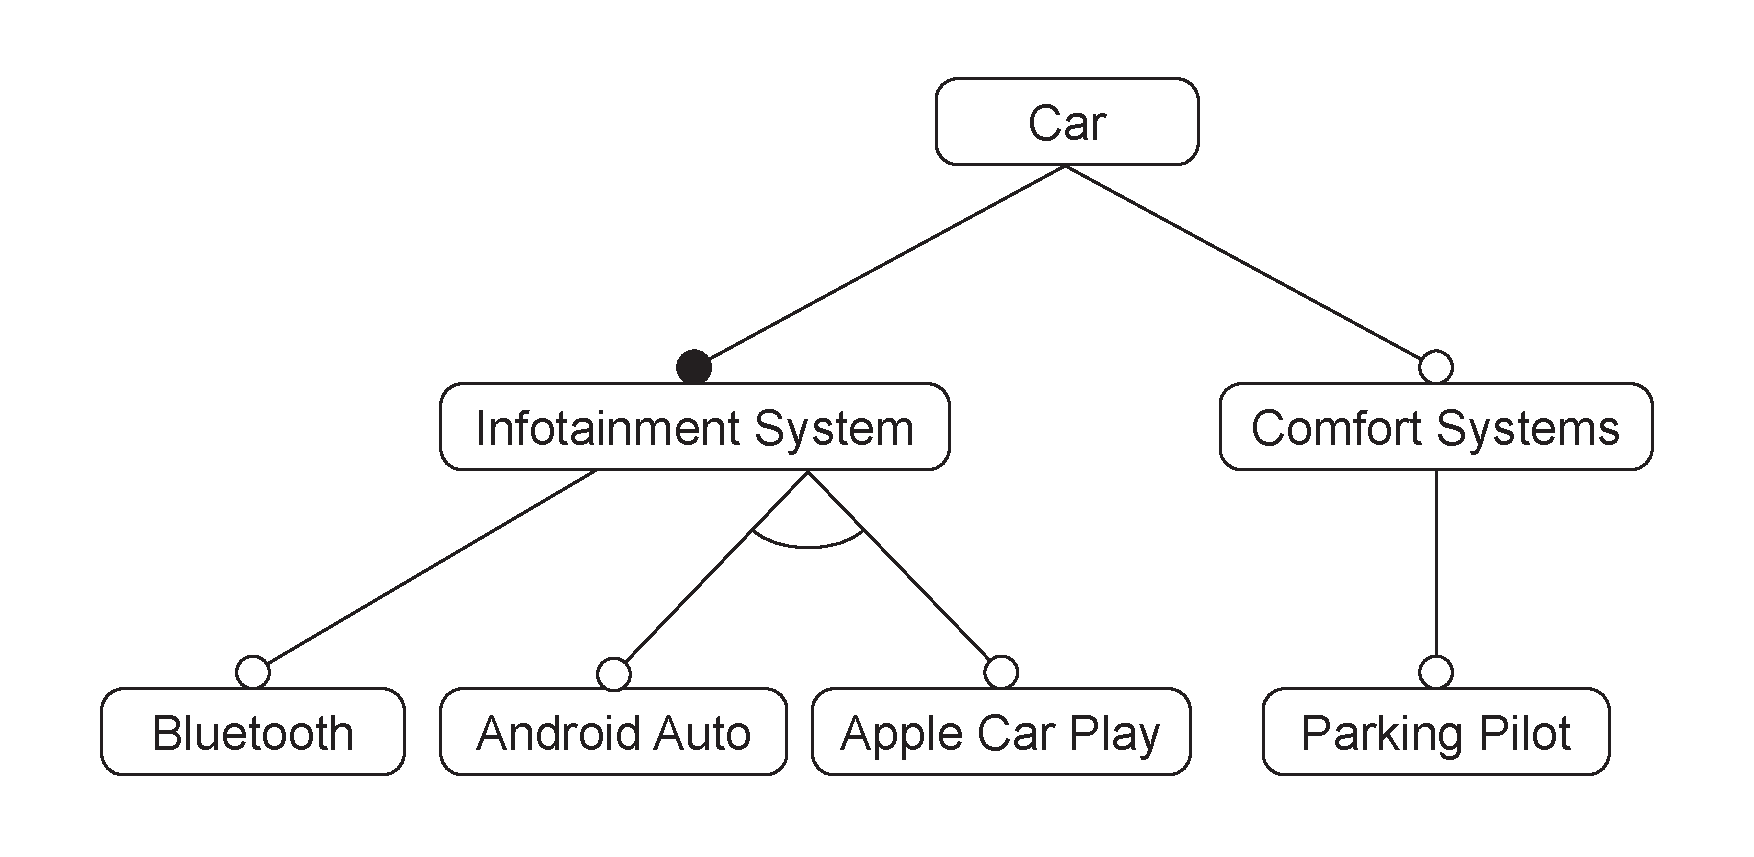
\includegraphics[width=0.8\linewidth]{illustrations/example.pdf}
	\caption{Example feature model}%
	\label{fig:example1}
\end{figure}

A visual representation of a feature model can be seen in Figure~\vref{fig:example1}. The small dot above \texttt{Infotainment System} indicates that the feature is mandatory, where as the white dot above \texttt{Comfort Systems} represents an optional feature. Each feature (except the root) is in a group. The \texttt{Infotainment System} feature is in a singleton group below \texttt{Car}. The features \texttt{Android Auto} and \texttt{Apple Car Play} are in a \texttt{XOR} group, indicated by the arch between the features. This represents that each valid variant has to choose between one of the two (but not both).

\section{Evolution planning}%
\label{sec:evolution_planning}

Feature models let engineers capture all variants of the current software product line, but sometimes it can be beneficial to model future or past versions as well. Planning for the long term evolution of the product line can be important in managing the complexity that comes with large software systems. Developing these kinds of systems typically involves many engineers, managers or other stakeholders, and managing when certain changes, additions or deprecations are implemented can be complex and confusing without suitable tools. Changing the SPL potentially influences many configurations, which might conflict with the stakeholders requirements.

SPL evolution is a major challenge in SPL engineering as many stakeholders are involved, many requirements exist, and changing the SPL potentially influences many configurations. Thus, it is paramount to thoroughly plan SPL evolution in advance, e.g., to perform analyses and to have enough time for implementing new or adapted features.

\textit{Evolution plans} lets us model a sequence of feature models, which represents the current and all planned future versions of the feature model. Each feature model represents the product line in a point in time, which could have varying validity, from a week from now to a year. Since the next feature model is derived from the previous one, we can represent the evolution plan as an initial feature model, as well as a sequence of \textit{points}, where each point is a set of operations to perform on the previous feature model to achieve the current one. The operations vary from changing, adding or deleting features or groups from the feature model.

\begin{figure}[htpb]
	\centering
	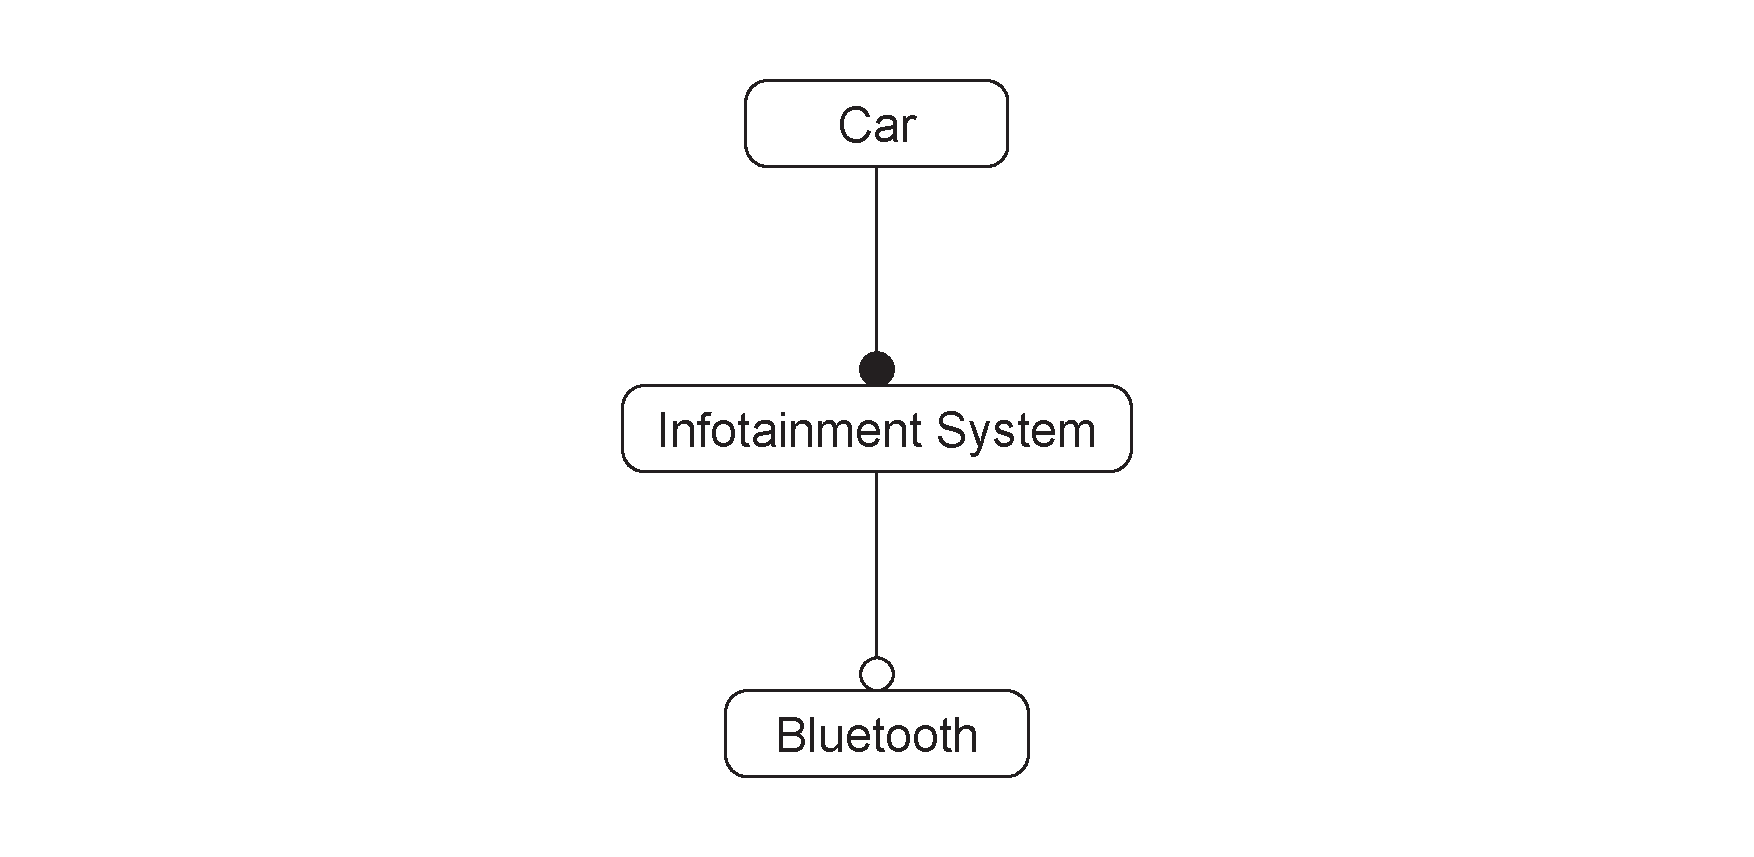
\includegraphics[width=0.8\linewidth]{illustrations/initial.pdf}
	\begin{tabular}{l}
		\textbf{At time 1:}                                           \\ \hline
		add an XOR group to Infotainment System.                      \\
		add feature Android Auto to the Infotainment System XOR group \\
		add feature Car Play to the Infotainment System XOR group     \\
		\\
		\textbf{At time 2:}                                           \\ \hline
		add feature Comfort Systems to the Car AND group              \\
		add an AND group to Comfort Systems                           \\
		add feature Parking Pilot to the Comfort Systems AND group
	\end{tabular}
	\caption{An example evolution plan}%
	\label{fig:exampleplan}
\end{figure}

An example of an evolution plan can be seen in Figure~\vref{fig:exampleplan}. The initial feature model contains three features, and two time points are added. At time 1, a group and two features are added, and at time 2, another group and two features are added. The evolution plan can derive three feature models, the initial, and the two at time 1 and 2. Performing all the operations results in a feature model that is equal to the one in Figure~\vref{fig:example1}

\section{Version Control Systems}%
\label{sec:version_control_systems}

\textit{Software configuration mechanisms} is the discipline of managing the evolution of large and complex software systems \cite{cite:software_configuration_management}. \textit{Version control mechanisms} are used to deal with the evolution of software products. These mechanisms include ways to deal with having multiple, parallel versions of the software simultaneously. Techniques like \textit{software merging} are used to keep consistency and unify different versions by automatically or semi-automatically deriving merged versions of the different parallel versions.

Mens~\cite{cite:tom_mens_software_merging_survey} categorizes and describes different aspect of version control systems and software merging techniques. Two-way and three-way merging differentiates between how many versions of the artifact you are comparing. Different representations of the merge artifact can be categorized in textual, syntactic, semantic or structural merging. State-based merge techniques uses delta algorithms to compute differences between revisions while change-based techniques keeps track of the exact operations that were performed between the revisions.

\subsection{Two-way vs three-way merging}%
\label{sub:two_way_vs_three_way_merging}

When merging different versions of a piece of software, we differentiate between \textit{two-way} and \textit{three-way} merging. Two-way merging merges the two versions without taking a common ancestor into account. Three-way merging on the other hand, uses a common ancestor as a reference point, to know how the different versions were changed. The latter technique is more powerful and produces more accurate merges, because the merge will know extra information from the common ancestor.

To illustrate the difference, consider the following program: \texttt{print(a); print(b); print(a + b)}, and two different versions derived from the base program, (1) \texttt{print(a); print(b); print(a+b); print("new line")}, (2) \texttt{print(b); print(a + b)}. Since a three-way merger uses the base program as a reference point, it will notice that derived version 1 added one statement, while version two deleted one. The three-way merger will then merge successfully without conflict with the following result: \texttt{print(b); print(a + b); print("new line")}. However, a two-way merger does not use the base program the different versions were derived from, and can not deduce whether \texttt{print(a)} were added in version 1 or deleted in version 2, thus raising a conflict. The same ambiguity occurs with the added statement \texttt{print("new line")}.

\subsection{Textual merging}%
\label{sub:textual_merging}

Textual merging views the software artifacts as unstructured text files. There exist several granularities of what is considered one unit, but \textit{line-based merging} is probably the most common textual merge. Line-based merging techniques computes the difference between files by comparing equality over the lines. This has several implications, like adding a single space after a line is considered a deletion of the old line and addition of the new. This coarse granularity often leads to unnecessary and confusing conflicts. Changing the indentation or other formatting differences often lead to unnecessary conflicts.

To exemplify this, consider the two versions of a Python program, Listing~\vref{lst:code_diff_1} and Listing~\vref{lst:code_diff_2}. The second version simply wrapped the content of the function in an if-statement that checks for input sanity. Using a standard textual, line-based differencing tool like the Unix' \textit{diff}-tool \cite{cite:fast_algo_for_lcs}, we are able to calculate the difference between the two files by calculating the longest common subsequence. As seen in the result (Listing~\vref{lst:result_code_diff}), difference between the two are confusing and inaccurate. Conceptually, the difference is that the second version wrapped the block in a if-statement. Due to the coarse grained line-based differencing and the disregard of structure and semantics, the algorithm reports that the whole block is deleted, and the same block wrapped in an if is inserted.

\begin{listing}
	\begin{minted}[]{python}
def some_function(n):
  sum = 0
  for i in range(0, n):
    sum += i
  print(sum)
some_function(5)

  \end{minted}
	\caption{Code diff 1}
	\label{lst:code_diff_1}
\end{listing}

\begin{listing}
	\begin{minted}[]{python}
def some_function(n):
  if isinstance(n, int):
    sum = 0
    for i in range(0, n):
      sum += i
    print(sum)
some_function(5)
  \end{minted}
	\caption{Code diff 2}
	\label{lst:code_diff_2}
\end{listing}

\begin{listing}
	\begin{minted}{text}
<   sum = 0
<   for i in range(0, n):
<     sum += i
<   print(sum)
---
>   if isinstance(n, int):
>     sum = 0
>     for i in range(0, n):
>       sum += i
>     print(sum)
  \end{minted}
	\caption{Resulting code diff}
	\label{lst:result_code_diff}
\end{listing}

As discussed, text-based merge techniques often provide inferior results, however, they have several advantages in terms of efficiency and generality. The algorithm is general enough to work well for different programming languages, documentation, markup files, configuration files, etc. Some measurements performed on three-way, textual, line-based merge techniques in industrial case studies showed that about 90 percent of the changed files could be merged automatically \cite{cite:large_scale_case_study}. Other tools can complement the merge algorithm in avoiding or resolving conflicts. Formatters can make sure things like indentation and whitespace are uniformly handled, to avoid unnecessary conflicts. Compilers can help in resolving conflicts arising from things like renaming, where one version renames a variables, while another version introduces new lines referencing the old variable.

\subsection{Syntactic Merging}%
\label{sub:syntactic_merging}

\textit{Syntactic merging}~\cite{cite:syntactic_software_merging} differs from textual merging in that it considers the syntax of the artifact it is merging. This makes it more powerful, because depending on the syntactic structure of the artifact, the merger can ignore certain aspects, like whitespace or code comments. Syntactic merge techniques can represent the software artifacts in a better data structure than just flat text files, like a tree or a graph. In example, representing the Python program from Listing~\vref{lst:code_diff_1} and Listing~\vref{lst:code_diff_2} as a parse tree or abstract syntax tree, we can avoid merge conflicts.

The granularity of the merger is still relevant, because we sometimes want to report a conflict even though the versions can be automatically merged. Consider the following example. $n < x$ is changed to $n \leq x$ in one version, and to $n < x + 1$ in another. Too fine grained granularity may cause this to be merged conflict free as $n \leq x + 1$. The merge can be done automatically and conflict free, but here we want to report a warning or conflict, because the merge might lead to logical errors.

\subsection{Semantic Merging}%
\label{sub:semantic_merging}

While syntactic merging is more powerful than its textual counterpart, there are still conflicts that go unnoticed. The syntactical mergers can detect conflicts explicitly encoded in the tree structure of the software artifact, however, there often exist implicit, cross-tree constraints in the software. An example of such a constraint is references to a variable. The variable references in the code are often semantically tied to the definition of the variable, where the name and scope implicitly notes the cross tree reference to the definition.

Consider the following simple program: \texttt{var i; i = 10;}. If one version changes the name of the variable: \texttt{var num; num = 10;}, and another version adds a statement referencing the variable: \texttt{var i; i = 10; print(i)}. Syntactic or textual mergers would not notice the conflict arising due to the implicit cross-tree constraints regarding the variable references, and merge the versions conflict-free with the following, syntactically valid result: \texttt{var num; num = 10; print(i)}.

Semantic mergers takes these kinds of conflicts into consideration while merging. Using \textit{Graph-based}  or \textit{context-sensitive} merge techniques, we can model such cross tree constraints, by linking definitions and invocations with edges in the graph. However, in some cases, such \textit{static semantic} merge techniques are not sufficient. Some changes cannot generally be detected statically, and may need to rely on the runtime semantics.

\section{Haskell and Algebraic Data Types}%
\label{sec:haskell_and_algebraic_data_types}

\todo{write about type synonyms, data types including records and sum types. show polymorphic data types. maybe something about deriving, maybe lens generation? etc. something about maybe? expressive and strict type system}

\section{Problem Definition}%
\label{sec:problem_definition}

\chapter{Formal Semantics of Feature Model Evolution Plans}%
\label{cha:formal_semantics_of_feature_model_evolution_plans}

As stated in \textbf{RQ2} in section~\vref{sec:research_questions}, we want design the merger in a way that guarantees a sound merge result. In order to do so, we need to have a clear, formal definition of the software artifact at hand, namely feature model evolution plans.

The formal structure and semantics of evolution plans are defined in a paper published in the Software Product Line Conference (SPLC)\footnote{https://splc.net/}, which I was fortunate enough to contribute to \cite{cite:consistency_preserving_evolution_planning}. The paper defines the evolution plan as an initial feature model, together with an ordered list of planning sections containing all edit operations that are scheduled for the same time point. The edit operations include addition and deletion of features and groups, as well as modifications to their fields, such as names or types. For every operation, we defined what makes an operation valid or invalid according to the formal definitions of feature models. 

In the work in this thesis, I will build upon, alter and extend the definitions and semantics of evolution plans defined in the other work I have contributed to. The semantics of editing operations were defined to create a soundness checker for evolution plans, which is used as a tool aiding replanning of evolution plans. However, since the focus of this thesis is to harmonize different alterations to evolution plan, we will need to adapt the evolution plan representation to fit this task.

\section{Issues with using a list-based approach}%
\label{sec:issues_with_using_a_list_based_approach}

In our work on creating a soundness checker for evolution plans, we used a representation where the ordering of the operations for a single point in time mattered. This list-based approach of grouping operations had several advantages regarding the formal definition of sound evolution plans as well as implementation-specific concerns. In defining what was considered a well-defined operation, we considered only the current feature model and the operation at hand. What order the user applied the operations did not really matter, as long as applying each operation resulted in a sound evolution plan.

However, when we design an approach to merging two evolution plans, the exact way each feature model in the evolution plan was derived is besides the point. The only thing the user sees are a list of feature models associated with time points. Exactly how the evolution plan was manipulated, and in what order each editing operation took place is not relevant for the user, so it should also not be relevant for the merge algorithm. As described in \textbf{RQ3} in section~\ref{sec:research_questions}, we want to produce merge results that are predictable and transparent. Having a list-based approach might make it hard to differentiate equal plans. Since there often is more than one way of going from one feature model to another, seemingly equal evolution plans might be represented differently.

Since part of the goal is to produce a sound result, we cannot simply rearrange the ordering of operations without complications. Some operations might be dependent on other operations, and rearranging the operations might result in an unsound plan. 

To counter these issues, one might naïvely find an standardized ordering of operations so one could sort the operations, or simply just store them as a set of operations instead of a list. However, as we will see, the order of the operations still matter, and changing the ordering can have varying effects. We observe three different ordering related scenarios for operations; non-dependent operations, dependent operations, and shadowed operations. By swapping the operations in a plan, you might achieve one of these scenarios. In the following sections, We investigate the scenarios in the following sections, which is also illustrated in Figure~\ref{fig:operation_swap_effect}.

\subsection*{Non-dependent Operations}%
\label{sub:non_dependent_operations}

In some cases, swapping the order of the operations in a time point has no effect on the resulting feature model. To exemplify this, take a simple feature model with two features and a group, organized in the following way: $\texttt{Root} \rightarrow \texttt{G1} \rightarrow \texttt{F1}$. In the following time point, there is scheduled a removal of feature \texttt{F1} as well as a name change for the root feature \texttt{Root} to \texttt{F0}. Applying both operations should yield the following feature model: $\texttt{F0} \rightarrow \texttt{G1}$. Since there is no structural or semantic relation between the operations, the order of when they are applied makes no difference. With the current list-based representation of a plan for a single time point, there are two ways of representing the changes. You could either schedule the removal of the \texttt{F1} feature first, or the name change of the root feature first. 

\begin{figure}[htpb]
  \centering
  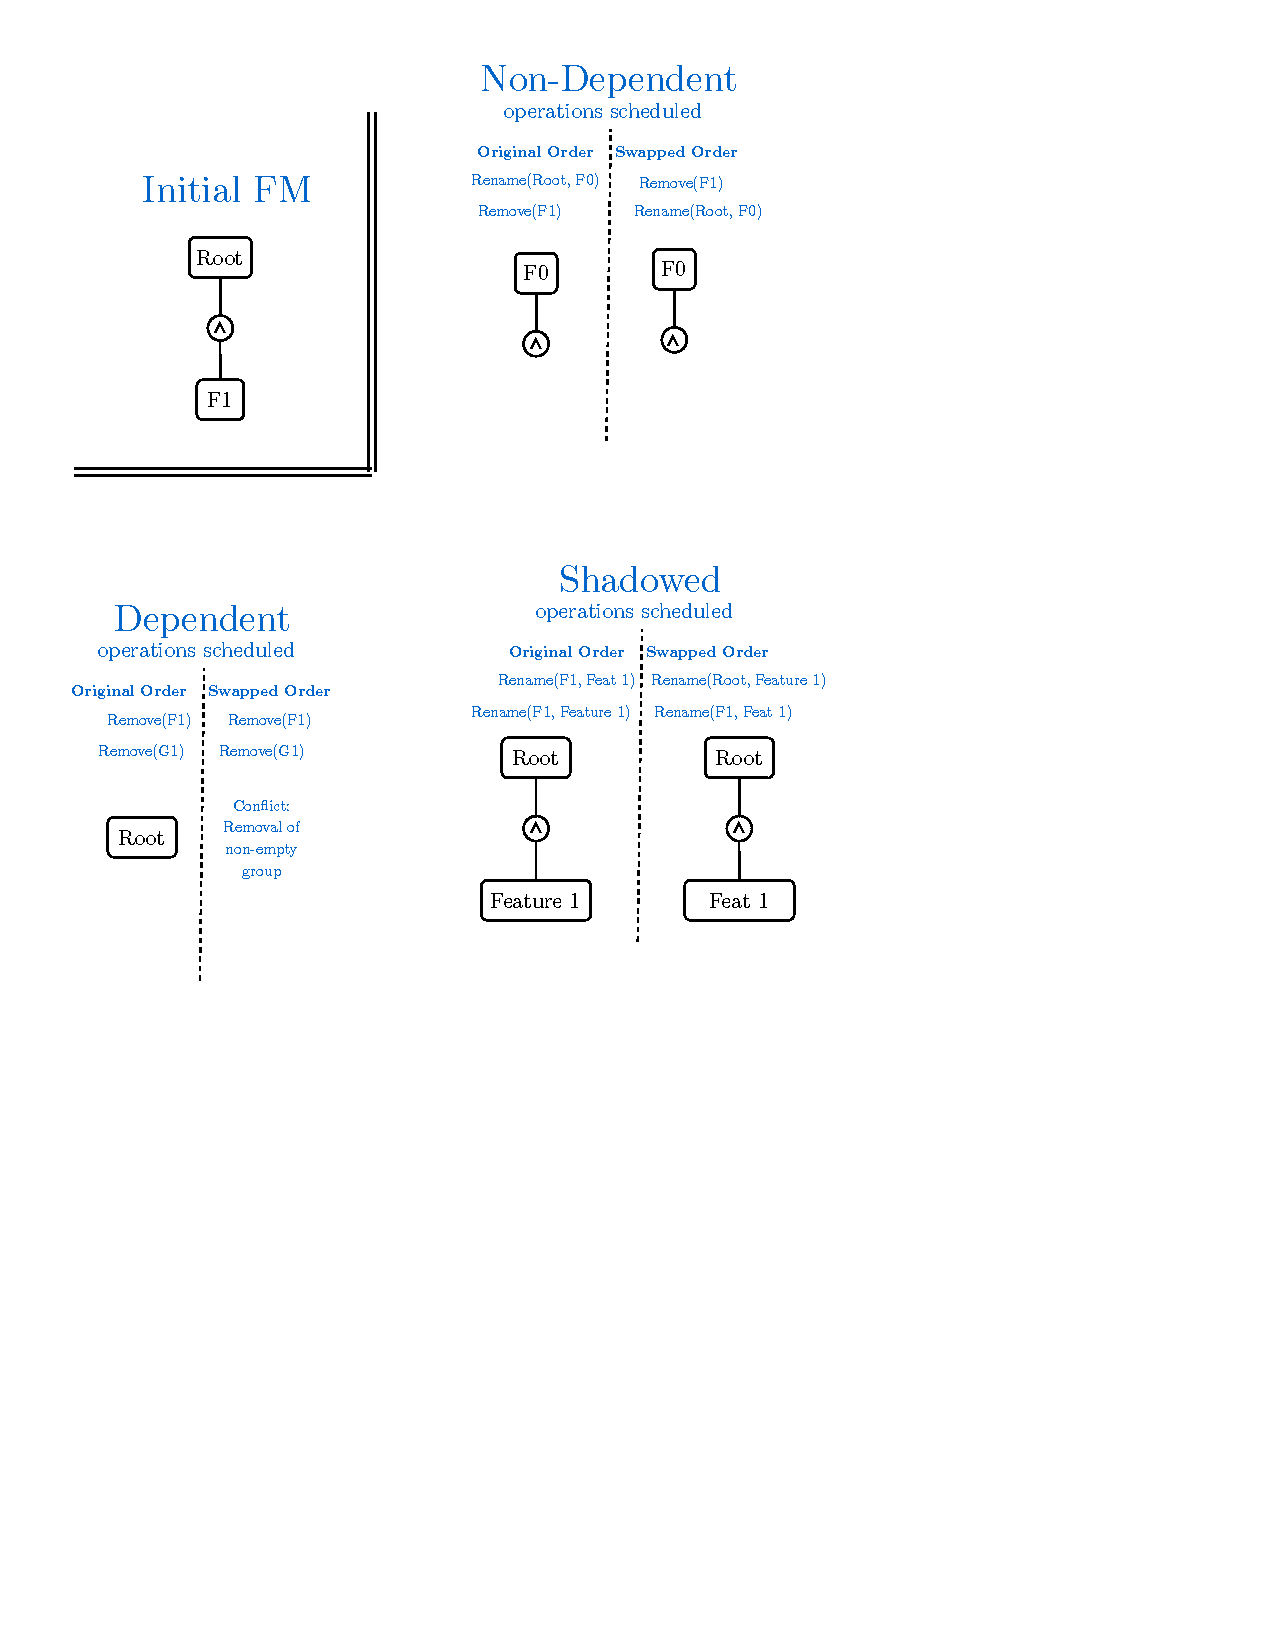
\includegraphics[width=0.8\linewidth]{operation_swap_effect.pdf}
  \caption{The various effects of swapping the ordering of operations}%
  \label{fig:operation_swap_effect}
\end{figure}

\subsection*{Dependent Operations}%
\label{sub:dependent_operations}

To showcase the problem, we start with the same feature model used previously, with two features and a group: $\texttt{Root} \rightarrow \texttt{G1} \rightarrow \texttt{F1}$. In the next planned time point, the changes to the feature model include the removal of both group \texttt{G1} and feature \texttt{F1}. However, there is only one legal ordering, namely removing the feature first, then removing the group. Applying the operation in this order yields a sound feature model; $\texttt{Root}$. Trying to remove the group first will as we defined sound evolution plans yield an inconsistency, because we are trying to remove a non-empty group. 

\subsection*{Operation Shadowing}%
\label{sub:operation_shadowing}

Another issue with the list-based approach is \textit{operation shadowing}, which is the phenomenon where an operation is rendered useless because of another operation later in the list. This issue would also have to be considered, because rearranging the operation could lead to unwanted results. In addition to rearrangement resulting in unsound plans, moving a shadowed operation might result in a different, yet sound evolution plan.

We exemplify operation shadowing, we consider the same initial feature model as before: $\texttt{Root} \rightarrow \texttt{G1} \rightarrow \texttt{F1}$. The list of operations for the next point in time include first changing the name of \texttt{F1} to \texttt{Feat 1}, then later to \texttt{Feature 1}. The operation shadowing occurs because of the second renaming makes the first renaming completely useless. The resulting feature model, $\texttt{Root} \rightarrow \texttt{G1} \rightarrow \texttt{Feature 1}$, are identical to the one we would have if we excluded the shadowed operation. However, if we were to swap the ordering of the rename operations, the resulting feature model would still be sound, but differ from the original ordering: $\texttt{Root} \rightarrow \texttt{G1} \rightarrow \texttt{Feat 1}$.

\section{Constructing a Normal Form for Evolution Plans}%
\label{sec:constructing_a_normal_form_for_evolution_plans}

In order to avoid the problems stated above, we construct a new representation for evolution plans. This representation is more aligned with what the user interacts with, so equal plans are also represented equally. In this representation, called \texttt{TreeUserEvolutionPlan}, the evolution plan is represented as a list of feature models together with a time point. Instead of storing the operations necessary to go from the previous time point to the next, each feature model is explicitly encoded. Each feature model is represented as a mutually recursive tree structure of features and groups. This representation is the normal form of evolution plans, and the closest representation to what the user actually interacts with.

The exact representation of \texttt{TreeUserEvolutionPlan} are defined formally in the Haskell code. Haskell's powerful type system with records and algebraic data types allows for a pretty precise formalization. When presented here in the thesis, the types are somewhat simplified, leaving out unnecessary noise, such as automatically derived instances for JSON serialization, equality checking, etc.

\subsection{Feature Model Definition - Tree Representation}%
\label{sub:feature_model_definition_tree_representation}

First, we will look at the tree representation for feature models, formalized as \texttt{TreeFeatureModel}.

\begin{minted}{haskell}
data TreeFeatureModel = TreeFeatureModel
  { rootFeature :: TreeFeature
  }

data TreeFeature = TreeFeature
  { id :: FeatureId
  , featureType :: FeatureType
  , name :: String
  , groups :: Set TreeGroup
  }

data TreeGroup = TreeGroup
  { id :: GroupId
  , groupType :: GroupType
  , features :: Set TreeFeature
  }

data FeatureType
  = Optional
  | Mandatory

data GroupType
  = And
  | Or
  | Alternative

type FeatureId = String

type GroupId = String
\end{minted}

There is a few important things to note in this representation. Each feature and groups id is unique across the entire feature model, which we will leverage when merging. Each feature and group can have an arbitrary number of children. The children is organized in a \texttt{Set}, not a \texttt{List}, noting that the ordering is irrelevant. In order for the feature model to be sound, some combination of parent group type and child feature types are prohibited. If a group is of type \texttt{Alternative} or \texttt{Or}, every child feature has to be of type \texttt{Optional}.

\subsection{Evolution Plan Definition - User Level, Tree Representation}%
\label{sub:evolution_plan_definition_user_level_tree_representation}

\subsubsection*{Polymorphic User Level Evolution Plan}%
\label{ssub:polymorphic_user_level_evolution_plan}

Now that we have a suitable definition feature models, we define evolution plans. In this representation, we want the evolution plans to mirror what the user interacts with, so we define the evolution plan as a list of feature models. In later stages of the merge algorithm, we will reuse this \textit{user level} definition of evolution plans, only with a different definition of feature models. This allows us to leverage Haskell's polymorphic type system, which spares us from defining it twice.

\begin{minted}{haskell}
data UserEvolutionPlan featureModel = UserEvolutionPlan
  { timePoints :: [TimePoint featureModel]
  }

type Time = Int

data TimePoint featureModel = TimePoint
  { time :: Time
  , featureModel :: featureModel
  }
\end{minted}

\subsubsection*{Instantiated User Level Evolution Plan (Tree Feature Model)}%
\label{ssub:instantiated_user_level_evolution_plan_tree_feature_model_}

Now that a generalized representation for evolution plans are defined, using a representation with a list of feature models, we can instantiate the polymorphic evolution plan to create our normal form, \texttt{TreeUserEvolutionPlan}. This is relatively straight forward, the only thing we have to do is replace the \texttt{featureModel} argument with our concrete feature model, namely \texttt{TreeFeatureModel}.

\begin{minted}{haskell}
type TreeUserEvolutionPlan = UserEvolutionPlan TreeFeatureModel
\end{minted}

\subsection{Example Representation}%
\label{sub:example_representation}

Now that we have defined the normal form for evolution plans formally, we will give a concrete example and how it is represented in this formalization. The example we will showcase is a small example containing three time points. The initial feature model at time 0 is simply just the root feature. The next time point at time 1 adds a new group and two features belonging to this group. The last time point removes one of the features and alters the name of the root and type of the group. A visualization of this simple evolution plan can be seen in Figure~\vref{fig:simpleep_treeuser}. Below is the Haskell code necessary for encoding this example.

\begin{minted}{haskell}
simpleExample :: TreeUserEvolutionPlan
simpleExample =
  UserEvolutionPlan
    [ TimePoint 0 fm0
    , TimePoint 1 fm1
    , TimePoint 2 fm2
    ]
  where
    fm0 =
      TreeFeatureModel
        ( TreeFeature
            "rootFeature"
            Mandatory
            "Feature 1"
            []
        )
    fm1 =
      TreeFeatureModel
        ( TreeFeature
            "rootFeature"
            Mandatory
            "Feature 1"
            [ TreeGroup
                "group"
                And
                [ TreeFeature
                    "feature2"
                    Optional
                    "Feature 2"
                    []
                , TreeFeature
                    "feature3"
                    Mandatory
                    "Feature 3"
                    []
                ]
            ]
        )
    fm2 =
      TreeFeatureModel
        ( TreeFeature
            "rootFeature"
            Mandatory
            "Root Feature"
            [ TreeGroup
                "group"
                Or
                [ TreeFeature
                    "feature2"
                    Optional
                    "Feature 2"
                    []
                ]
            ]
        )
\end{minted}

Note that each feature and groups \texttt{Set} of children are constructed using list syntax. This is to make it a bit easier to read, not having too much visual clutter. This is possible using the language extension \texttt{OverloadedLists} \footnote{https://ghc.gitlab.haskell.org/ghc/doc/users\_guide/exts/overloaded\_lists.html}, where we allow Haskell's type system to figure out that the list is actually a \texttt{Set} based on the context.

\begin{figure}[htpb]
  \centering
  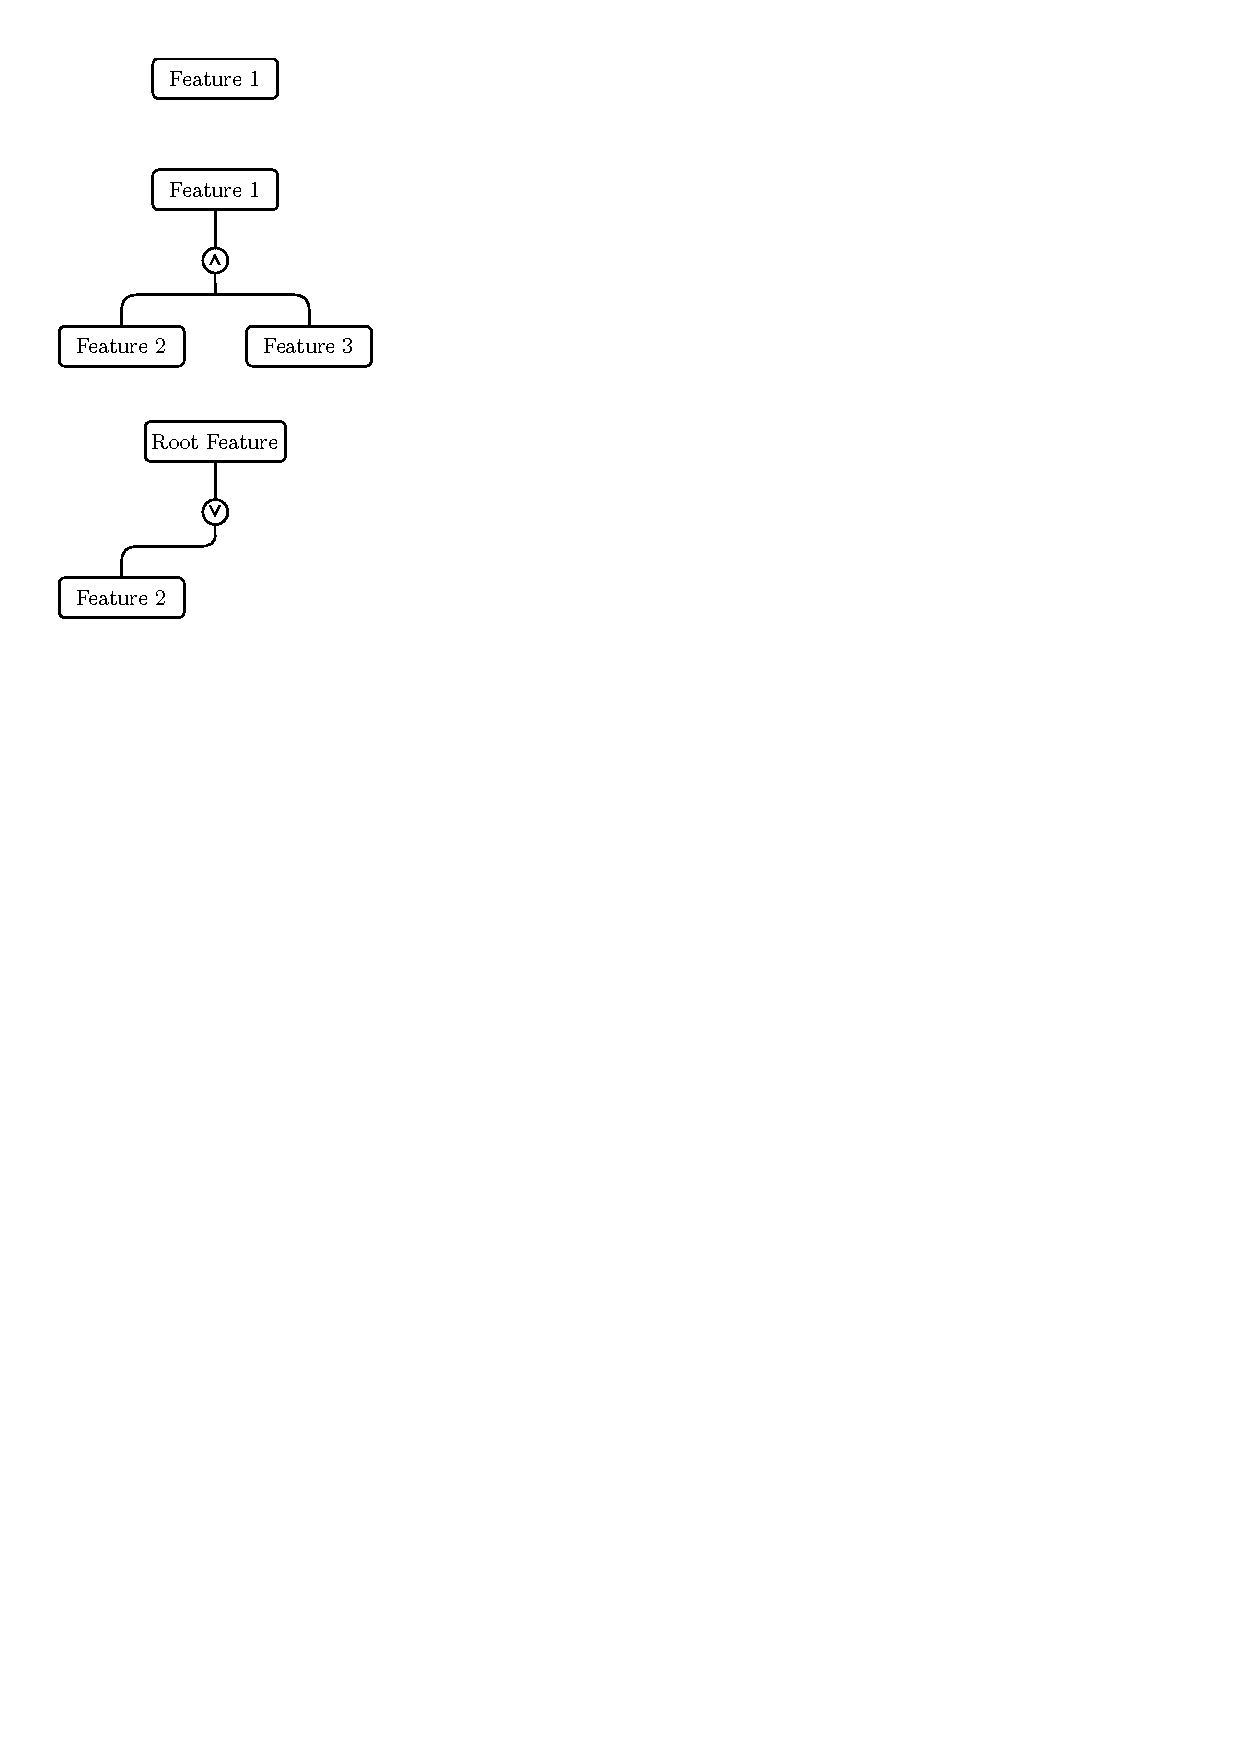
\includegraphics[]{simpleep_treeuser.pdf}
  \caption{A Simple Evolution Plan Example}%
  \label{fig:simpleep_treeuser}
\end{figure}

\section{A Suitable Representation of Evolution}%
\label{sec:a_suitable_representation_of_evolution}

The evolution plan formalization defined above, \texttt{TreeUserEvolutionPlan}, works well for capturing the essence of evolution plans. It represents evolution plans in terms of what the user actually deals with. However, in order to do an effective merge of two evolution plans, we need to represent the evolution plan a bit differently.

Refactoring the evolution plan doesn't just involve modifying the last time point, but replanning the other time points earlier in the plan. When users are replanning such time points, the additions, deletions and modifications has an effect not just on the time point at hand, but all subsequent time points. When a user adds a new feature in the middle of the plan, the feature would appear on the specified time points as well as all the time points beyond. When calculating the changes made, we don't want to look at this like a feature was added in all the time points, but rather just the specified time. In order to capture the essence of the changes made to each evolution plan, we would need to find a representation capturing the actual changes more explicitly.

In order to to capture the explicit modifications between each time point in the evolution plan, we would need to figure out an approach to calculating the difference between two subsequent feature models. However, with our current tree-based feature model, \texttt{TreeFeatureModel}, this can be a bit cumbersome, requiring us to traverse the two trees simultaneously. In some cases this is not very straight forward, i.e. handling \texttt{Move}-operations that relocates entire subtrees.

\subsection{Feature Model Definition - Flat Representation}%
\label{sub:feature_model_definition_flat_representation}

We define a new representation for feature models, \texttt{FlatFeatureModel}, in order to have a structure better suited for detecting and applying changes to the tree-structure. This is achievable due to our features and groups having unique ids. This allows for a simple mapping-structure, where we each feature and group can be looked up by its id. The edges and relations in the tree are modeled as node-id references instead of a recursive structure. Every node only stores its parent relation, not its child relations as well. This makes moving entire subtrees straight forward, requiring changing only the parent-field of the node to move.

\begin{minted}{haskell}
data FlatFeatureModel = FlatFeatureModel
  { rootId :: FeatureId
  , features :: Map FeatureId FlatFeature
  , groups :: Map GroupId FlatGroup
  }

data FlatFeature = FlatFeature
  { parentGroupId :: Maybe GroupId
  , featureType :: FeatureType
  , name :: String
  }

data FlatGroup = FlatGroup
  { parentFeatureId :: FeatureId
  , groupType :: GroupType
  }
\end{minted}

The definitions of \texttt{FeatureType}, \texttt{FeatureId}, \texttt{GroupType} and \texttt{GroupId} is still the same as defined in Section~\vref{sub:feature_model_definition_tree_representation}.

\subsection{Evolution Plan Definition - User Level, Flat Representation}%
\label{sub:evolution_plan_definition_user_level_flat_representation}

With our new, flat representation for feature models, we can use this to create a new user level representation, with our flat structure instead of the tree-based. Since we created a generalized data type, \texttt{UserEvolutionPlan}, we can instantiate it in the following way.

\begin{minted}{haskell}
type FlatUserEvolutionPlan = UserEvolutionPlan FlatFeatureModel
\end{minted}

With this new representation for evolution plans, the example from Figure~\vref{fig:simpleep_treeuser} can be encoded in the following way:

\begin{minted}{haskell}
simpleExampleFlat :: FlatUserEvolutionPlan
simpleExampleFlat =
  UserEvolutionPlan
    [ TimePoint 0 fm0
    , TimePoint 1 fm1
    , TimePoint 2 fm2
    ]
  where
    fm0 =
      FlatFeatureModel
        "rootFeature"
        [
          ( "rootFeature"
          , FlatFeature Nothing Mandatory "Feature 1"
          )
        ]
        []

    fm1 =
      FlatFeatureModel
        "rootFeature"
        [
          ( "feature2"
          , FlatFeature (Just "group") Optional "Feature 2"
          )
        ,
          ( "feature3"
          , FlatFeature (Just "group") Mandatory "Feature 3"
          )
        ,
          ( "rootFeature"
          , FlatFeature Nothing Mandatory "Feature 1"
          )
        ]
        [("group", FlatGroup "rootFeature" And)]
    fm2 =
      FlatFeatureModel
        "rootFeature"
        [
          ( "feature2"
          , FlatFeature (Just "group") Optional "Feature 2"
          )
        ,
          ( "rootFeature"
          , FlatFeature Nothing Mandatory "Root Feature"
          )
        ]
        [("group", FlatGroup "rootFeature" Or)]
\end{minted}

Each feature model in the evolution plan consists of a reference to the root feature id, as well as two \texttt{Map}s. Using the \texttt{OverloadedLists} extension, each Map is noted by a list of tuples, where the first part of the tuple is the id of the feature or group, and the second part is the fields of the feature or group.

\subsubsection*{Advantages over the tree structured evolution plan}%
\label{ssub:advantages_over_the_tree_structured_evolution_plan}

The new definition of feature models has advantages we will make deriving and integrating modifications between two subsequent feature models easier. 

Since we have a flat structure, deriving or integrating modifications on a feature or group saves us from traversing the tree structure. The flat structure leverages the unique ids in order to allow lookup based on id. Changing a feature or group requires a lookup based on the id, then changing the fields of the mapping entry. Removing or adding a node is similarly simple, requiring only adding or removing an entry in the mapping. Since the edges in the tree are modeled as references to the parent id, we don't need to modify the parent node when removing a node.

The flexible flat structure allows for temporarily damaging the tree-structure, which allows for applying modifications in an arbitrary order. We recall some of the issues related to the list-based operations in Section~\ref{sec:issues_with_using_a_list_based_approach}, where some dependent operations had to be applied in a specific order, i.e. adding the parent feature before adding the child group. Since the tree-structure of our \texttt{FlatUserEvolutionPlan} is implicit through the node-id references, we could simply add the child feature first, with a reference to the parent id, then directly after add the parent id. We just have to ensure that all the operations we apply will result in a sound feature model.

\subsection{Evolution Plan Definition - Modification Level, Flat Representation}%
\label{sub:evolution_plan_definition_modification_level_flat_representation}

As discussed in Section~\ref{sec:issues_with_using_a_list_based_approach}, the list-based operation approach is problematic in order to achieve a desired merge result. What the user perceived as equal plans had several representations. In order to combat this we created a normal form for evolution plans, \texttt{TreeUserEvolutionPlan}, more aligned with the users perspective of evolution plans. Since tree-based structure of its feature models had some disadvantages in terms of detecting and applying modifications, we created a new representation for feature models, which we used in our intermediate representation for evolution plans, \texttt{FlatUserEvolutionPlan}.

However, the user level evolution plan representation with the list of feature models for each time point didn't model the replanning aspect of evolution plans as we wanted. When users have to go back to intermediate time points in the evolution plan and make changes, the changes will appear in the subsequent time points as well. This requires modeling the evolution plan similar to the list-based operation approach discussed previously, while still avoiding the issues regarding operation ordering, operation shadowing, etc.

We present the final evolution plan representation, \texttt{FlatModificationEvolutionPlan}, modeling the evolution plan as an initial model along with an ordered list of time points associated with \textit{modifications}. The modifications model the changes necessary to go from the previous feature model to the one in the specified time point. The modifications consists of two mappings, one for features and one for groups. Each mappings map ids to a \textit{modification}. A modification can be one of three things, an addition, deletion or a change to one or more fields.

The Haskell representation of our \texttt{FlatModificationEvolutionPlan} can be seen below.

\begin{minted}{haskell}
data TransformationEvolutionPlan transformation featureModel = 
  TransformationEvolutionPlan
    { initialTime :: Time
    , initialFM :: featureModel
    , plans :: [Plan transformation]
    }

data Plan transformation = Plan
  { timePoint :: Time
  , transformation :: transformation
  }

type ModificationEvolutionPlan featureModel = 
  TransformationEvolutionPlan Modifications featureModel

type FlatModificationEvolutionPlan = 
  ModificationEvolutionPlan FlatFeatureModel
\end{minted}

Notice that the actual types are generalized in two ways. As with our user level representation, we have made the evolution plan polymorphic over the feature model. In addition, we have generalized the actual transformation type necessary to go from one feature model to the next. This is useful for the actual merge algorithm, which will reuse the evolution plan with another transformation type. With the evolution plan structure in place and our newly defined \texttt{ModificationEvolutionPlan}, we can define \texttt{Modifications} in the following way:

\begin{minted}{haskell}
data Modifications = Modifications
  { features :: Map FeatureId FeatureModification
  , groups :: Map GroupId GroupModification
  }

data FeatureModification
  = FeatureAdd GroupId FeatureType String
  | FeatureRemove
  | FeatureModification
      (Maybe FeatureParentModification)
      (Maybe FeatureTypeModification)
      (Maybe FeatureNameModification)

data FeatureParentModification
  = FeatureParentModification GroupId

data FeatureNameModification
  = FeatureNameModification String

data FeatureTypeModification
  = FeatureTypeModification FeatureType

data GroupModification
  = GroupAdd FeatureId GroupType
  | GroupRemove
  | GroupModification
      (Maybe GroupParentModification)
      (Maybe GroupTypeModification)

data GroupParentModification
  = GroupParentModification FeatureId

data GroupTypeModification
  = GroupTypeModification GroupType
\end{minted}

\subsubsection*{Example representation}%
\label{ssub:example_representation}

With our final, merge ready representation of evolution plans, we can encode the simple example in the defined data types. A visual representation of the example can be seen in Figure~\ref{fig:simpleep_flatmod}

\begin{minted}{haskell}

simpleExampleMod :: FlatModificationEvolutionPlan
simpleExampleMod =
  TransformationEvolutionPlan
    0
    initial
    [Plan 1 modifications1, Plan 2 modifications2]
  where
    initial =
      FlatFeatureModel
        "rootFeature"
        [
          ( "rootFeature"
          , FlatFeature Nothing Mandatory "Feature 1"
          )
        ]
        []
    modifications1 =
      Modifications
        [
          ( "feature2"
          , FeatureAdd "group" Optional "Feature 2"
          )
        ,
          ( "feature3"
          , FeatureAdd "group" Mandatory "Feature 3"
          )
        ]
        [("group", GroupAdd "rootFeature" And)]
    modifications2 =
      Modifications
        [ ("feature3", FeatureRemove)
        ,
          ( "rootFeature"
          , FeatureModification
              Nothing
              Nothing
              (Just (FeatureNameModification "Root Feature"))
          )
        ]
        [
          ( "group"
          , GroupModification
              Nothing
              (Just (GroupTypeModification Or))
          )
        ]
\end{minted}

\begin{figure}[htpb]
  \centering
  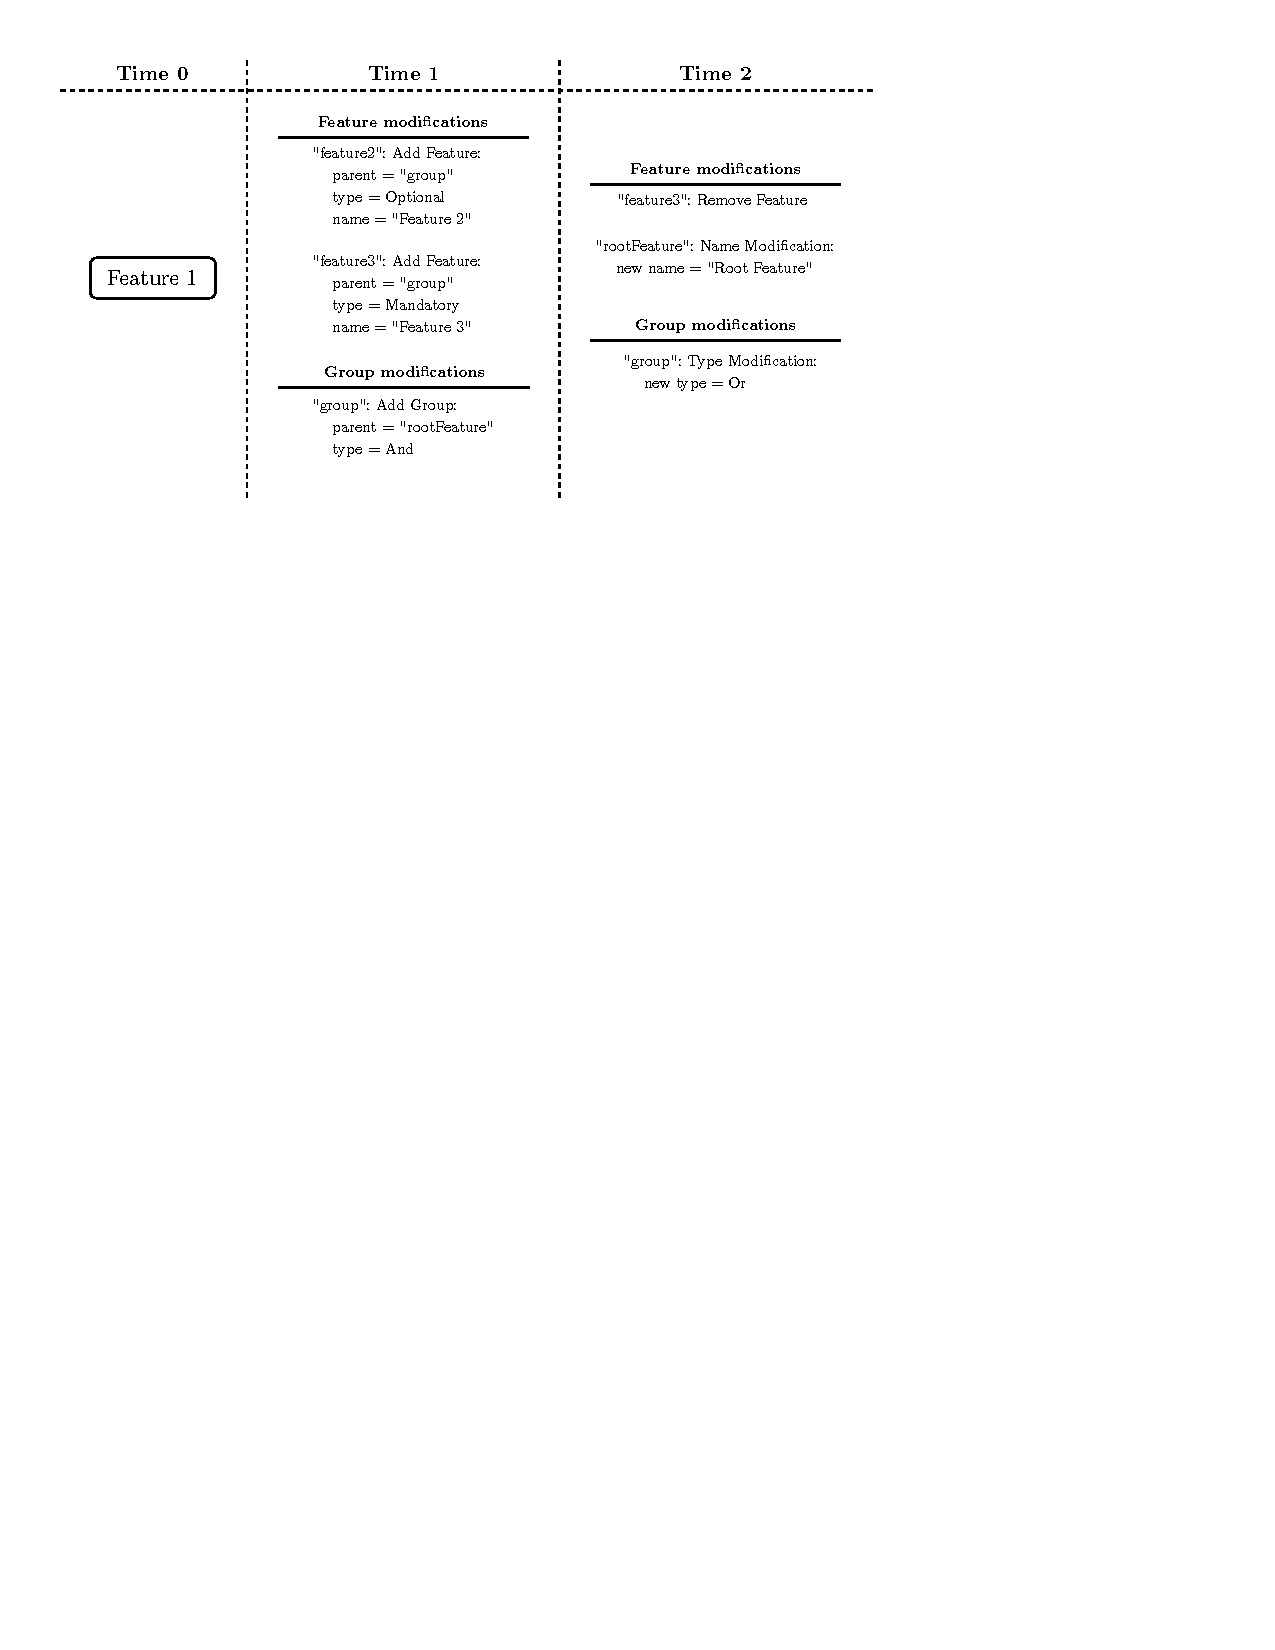
\includegraphics[]{simpleep_flatmod.pdf}
  \caption{A Simple Evolution Plan Example}%
  \label{fig:simpleep_flatmod}
\end{figure}

% An important part in merging the efforts of two collaborators is figuring out exactly what changes each collaborators did to the common base evolution plan. With our current representation of evolution plans, \texttt{TreeUserEvolutionPlan}, detecting changes in the tree can be quite difficult.




\todo{kan snakke om operasjonene, hva de betyr på høynivå. referere til artikkel for detaljer.}
\todo{arbeid er basert på sunn plan.}

\chapter{Three Way Merge Algorithm}%
\label{cha:three_way_merge_algorithm}

\section{Algorithm Overview}%
\label{sec:algorithm_overview}

\subsection{Three-Way Merging of Evolution Plans}%
\label{sub:three_way_merging_of_evolution_plans}

The three-way merge algorithm for feature model evolution plans will take two different versions of an evolution plan, \textit{version 1} and \textit{version 2}, and attempt to merge the evolution plans into a single plan. In order to do so, a third evolution plan has to be provided, which is the common evolution plan they were derived from. The common evolution plan, called \textit{base}, will implicitly provide information about what things were added, removed and changed in each of the derived evolution plans.

\subsection{Soundness Assumption}%
\label{sub:soundness_assumption}

The three-way merge algorithm will assume that the three evolution plans provided are sound. By assuming the soundness of the plans, the algorithm can leverage this to create a better merge result. But more importantly, the assumption is based around the fact that there is no point in merging an evolution plan you know violates soundness in some way.

\subsection{Algorithm Phases}%
\label{sub:algorithm_phases}

In order to merge the different versions of the evolution plan, the algorithm is separated into several distinct phases. The different steps and phases of the algorithm can be seen in Figure~\ref{fig:merge_outline}.

\begin{figure}[htbp]
  \centering
  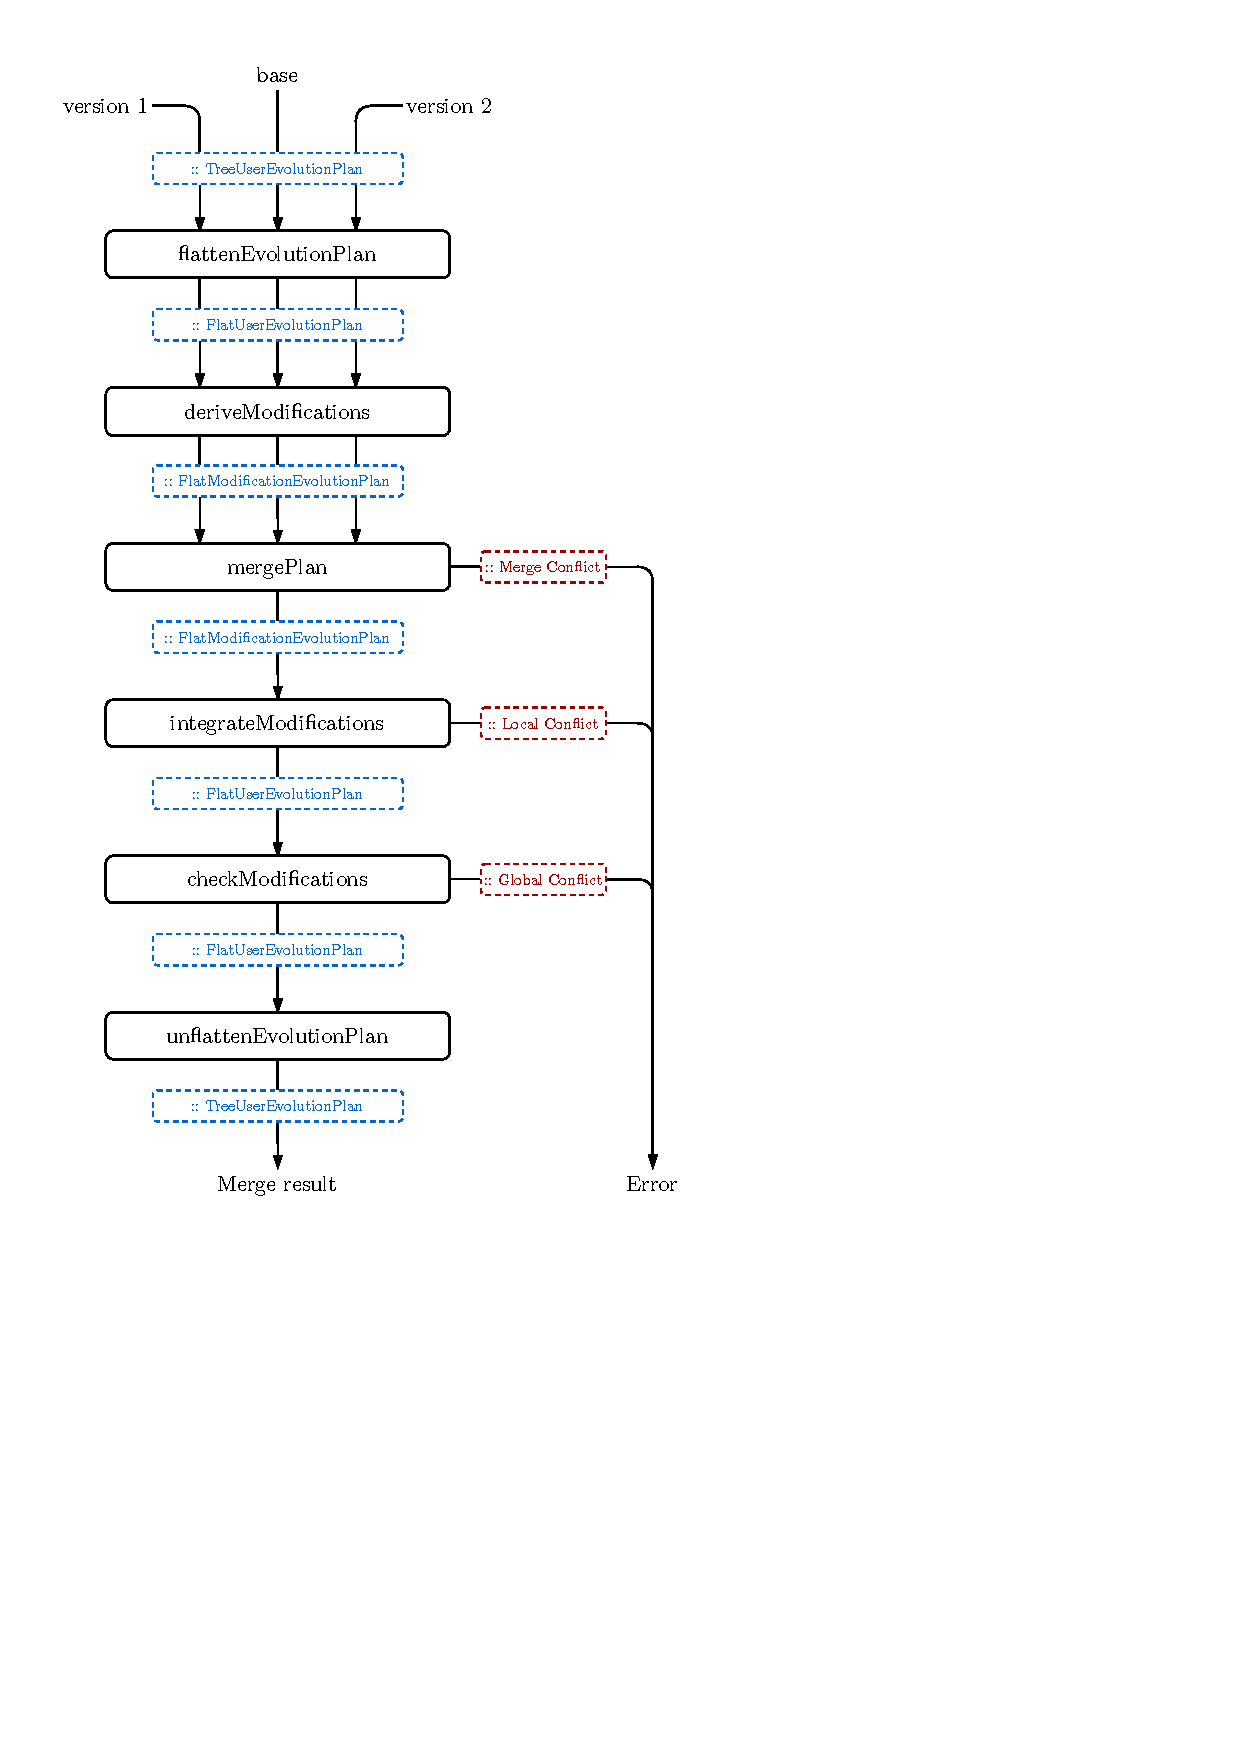
\includegraphics[width=0.8\linewidth]{merge_outline}
  \caption{Outline of the three-way merge algorithm}%
  \label{fig:merge_outline}
\end{figure}

The first phase is transforming the three different evolution plans into representations that is more suitable for merging. This includes converting both the way feature models are represented as well as the way the entire evolution plan is represented. This phase includes the \texttt{flattenEvolutionPlan} and \texttt{deriveModifications}, which is described in further detail in \vref{sec:converting_to_a_suitable_representation}

After changing the way evolution plans are represented, the second phase of the algorithm will calculate the differences between the \textit{base} evolution plan and both derived evolution plans, \textit{version 1}, and \textit{version 2}. This will let us know what were added, changed and removed in each of the derived evolution plans. This phase is part of the \texttt{mergePlan} function, which is described in further detail in \vref{sec:detecting_the_changes_between_versions}

The information from the previous phase will be used to create a single merged evolution plan. This evolution plan is simply just the \textit{base} evolution plan integrated with all the changes from \textit{version 1} and \textit{version 2}. This phase is part of the \texttt{mergePlan} function, which is described in further detail in \vref{sec:merging_intended_changes}

Now that a single merged evolution plan is provided, the last step is to ensure that the plan is following the structural and semantic requirements of an evolution plan. Merging all changes from both versions might yield various inconsistencies. This includes structural conflicts such as orphan features, entire subtrees forming cycles, removing non-empty features, etc. The last phase includes converting back to the original representation, as well as ensuring soundness while doing so. This phase is part of the \texttt{integrateModifications}, \texttt{checkModifications} and \texttt{unflattenEvolutionPlan} functions, which is explained further in \vref{sec:ensuring_structural_and_semantic_soundness_of_merge_result}

\subsection{Conflicts}%
\label{sub:conflicts}

During the different phases of the merge algorithm, different kind of conflicts or errors could occur. Depending on what part of the algorithm a conflict occurred, the conflicts might be either a \textit{merge}, \textit{local} or \textit{global} conflict. At what phase each conflict could occur can also be seen in Figure~\vref{fig:merge_outline}, but a short description of the different conflicts are described below. 

\textit{Merge Conflicts} occur because of conflicting operations on a single feature or group. This could happen if one version tries to remove a feature, while the other tries to change the type of a feature. This could also happen if there originally existed a modification in the \textit{base} version, and one of the derived versions try to change the modification, while the other tries to remove the modification.

\textit{Local Conflicts} occur when a modification is not possible to be applied because of the existence or non-existence of a feature or group. For example, if we try to add a feature with an id that already exist, or try to change the type of a group that does not exist.

\textit{Global Conflicts} is the last kind of error that could occur. When all the modifications has been integrated into the evolution plan, each feature model is checked for certain structural or semantical errors. At this point, each change \textit{local} to a feature or group is valid, so we check for potential errors that occur because of dependencies between the features and groups, \textit{global} to the entire feature model. The structural errors is typically modifications that lead to anomalies in the tree structure. These violations of the structure could happen if you add features to parents that don't exist, remove groups that has children, or move features in such a way that cycles are formed. Other violations to the semantics are also checked. This could for example be violations of well-formedness, that could happen if we change the type of a feature to something incompatible with its group.

\section{Converting To a Suitable Representation}%
\label{sec:converting_to_a_suitable_representation}

As discussed in Chapter~\ref{cha:formal_semantics_of_feature_model_evolution_plans}, we needed to create a suitable representation for evolution plans before attempting to merge the different versions.

The input of the three-way merge algorithm is three evolution plans in our evolution plan normal form, \texttt{TreeUserEvolutionPlan}. Each of the three evolution plans will be transformed into our merge-ready representation of evolution plan in two steps. First we will use \texttt{flattenEvolutionPlan} in order to flatten the evolution plan and represent it as our intermediate representation \texttt{FlatUserEvolutionPlan}. After this transformation, the evolution plans will be transformed into the merge-ready representation, \texttt{FlatModificationEvolutionPlan}.

\subsection{Transformation to the Intermediate Representation}%
\label{sub:transformation_to_the_intermediate_representation}

The first step in the merge algorithm is using \texttt{flattenEvolutionPlan} to transform the tree-based evolution plan into the flattened structure. Note that in the code we call this \texttt{flattenSoundEvolutionPlan}, since we assume that the three plans in the algorithm is sound. In order to do this transformation, we would need to go through every feature model in the plan and transform it using \texttt{flattenSoundFeatureModel}

\begin{minted}[breaklines]{haskell}
flattenSoundEvolutionPlan :: 
  TreeUserEvolutionPlan -> 
  FlatUserEvolutionPlan
flattenSoundEvolutionPlan =
  L.timePoints
    . traversed
    . L.featureModel
    %~ flattenSoundFeatureModel
\end{minted}

Flattening a feature model is relatively straight forward, requiring traversing the tree structure, and creating a list of features and a list of groups as we traverse. In order to do so, we create a tuple of lists, where the left side contains a list of flat features and the right side a list of flat groups. When traversing the tree, we create a new flat feature or group, and concatinate it with the result from the recursive call with \texttt{<>} and \texttt{foldMap}.

\begin{minted}[breaklines]{haskell}
flattenSoundFeatureModel :: 
  TreeFeatureModel -> 
  FlatFeatureModel
flattenSoundFeatureModel fm =
  FlatFeatureModel
    (fm ^. L.rootFeature . L.id)
    (M.fromList features)
    (M.fromList groups)
  where
    (features, groups) = 
      flattenFeature Nothing (fm ^. L.rootFeature)
    flattenFeature parent (TreeFeature id fType name gs) =
      ([(id, FlatFeature parent fType name)], [])
        <> foldMap (flattenGroup id) gs
    flattenGroup parent (TreeGroup id gType fs) =
      ([], [(id, FlatGroup parent gType)])
        <> foldMap (flattenFeature (Just id)) fs
\end{minted}

\subsection{The Final, Merge Ready Representation}%
\label{sub:the_final_merge_ready_representation}

After transforming to our intermediate representation, we begin the process of deriving the modifications between each pair of subsequent feature models. As before, we have assumed soundness for our plans, which is why the actual function in the code is called \texttt{deriveSoundModifications} and not \texttt{deriveModifications} as in Figure~\ref{fig:merge_outline}.

The function will use the first time point in the evolution plan as the initial time point, and create a list of subsequent feature model pairs which is then passed to the \texttt{timePointsToPlan} function. The function will use the two subsequent feature models, previous and current, to calculate the differences between them.

\begin{minted}[breaklines]{haskell}
deriveSoundModifications :: 
  FlatUserEvolutionPlan -> 
  FlatModificationEvolutionPlan
deriveSoundModifications (UserEvolutionPlan timePoints) = 
  case timePoints of
    [] -> error $ "evolution plan has to have " 
               ++ "at least one time point!"
    ((TimePoint initialTime initialFM) : restTimePoints) ->
      TransformationEvolutionPlan
        initialTime
        initialFM
        (zipWith timePointsToPlan timePoints restTimePoints)

timePointsToPlan ::
  TimePoint FlatFeatureModel -> 
  TimePoint FlatFeatureModel -> 
  Plan Modifications
timePointsToPlan 
  (TimePoint _ prevFM) 
  (TimePoint currTime currFM) =
    Plan currTime $ diffFeatureModels prevFM currFM
\end{minted}

The main part of the algorithm is actually detecting the changes between the two feature models and representing them in the \texttt{Modifications} data type. The function defined below, \texttt{diffFeatureModels}, handles this process. Since the flat representation of feature models includes two maps, one for features and one for groups, we calculate the modifications for both separately using the functions \texttt{calculateFeatureModifications} and \texttt{calculateGroupModifications}.

\begin{minted}[breaklines]{haskell}
diffFeatureModels :: 
  FlatFeatureModel -> 
  FlatFeatureModel -> 
  Modifications
diffFeatureModels prevFM currFM =
  Modifications
    ( calculateFeatureModifications
        (prevFM ^. L.features)
        (currFM ^. L.features)
    )
    ( calculateGroupModifications
        (prevFM ^. L.groups)
        (currFM ^. L.groups)
    )
\end{minted}

In order to calculate the differences between two \texttt{Map}s, we rely on the Haskell module \texttt{Data.Map.Merge} from the containers module\footnote{https://hackage.haskell.org/package/containers-0.6.2.1}. This module provides ways of merging maps with keys of the same type. In our case, we have two mappings from \texttt{FeatureId} to \texttt{FlatFeature}, which we will attempt to merge into a mapping from \texttt{FeatureId} to \texttt{FeatureModification}. The merging will be done using the \texttt{merge} function from \texttt{Data.Map.Merge}, which will compare the keys, the feature ids, in both maps. Based on the result of the comparison, one of three different merge tactics will be used to produce the desired result. The merge tactics will rely on the three functions that we pass to the \texttt{merge} function. Given a feature id, the following three cases describes can appear:

\begin{itemize}
  \item \textbf{The id exists only in the previous feature model}: This will produce a \texttt{FeatureRemove} modification for the id.
  \item \textbf{The id exists only in the next feature model}: Since the feature did not exist in the previous feature model, but appeared in this, we will get a \texttt{FeatureAdd} modification for the id.
  \item \textbf{The id exists in both the previous and next feature models}: If the two features are equal, no modification should be generated. However, if any of the fields has changed, a \texttt{FeatureModification} would be generated. The modification will include all the fields that were changed, and skip the ones that remained unchanged.
\end{itemize}

\begin{minted}[breaklines]{haskell}
calculateFeatureModifications ::
  Map FeatureId FlatFeature ->
  Map FeatureId FlatFeature ->
  Map FeatureId FeatureModification
calculateFeatureModifications =
  Merge.merge
    (Merge.mapMissing (const inPrev))
    (Merge.mapMissing (const inNew))
    (Merge.zipWithMaybeMatched (const inBoth))
  where
    inPrev _ = FeatureRemove
    inNew (FlatFeature mParent featureType name) =
      case mParent of
        Nothing -> error "cannot add a new root"
        Just parent -> FeatureAdd parent featureType name
    inBoth prev new =
      let FlatFeature prevParent prevType prevName = prev
          FlatFeature newParent newType newName = new
       in if prev == new
            then Nothing
            else Just $
              FeatureModification
                ( case (prevParent, newParent) of
                    (Just prev, Just new)
                      | prev /= new ->
                        Just (FeatureParentModification new)
                    -- NOTE: since the root is assumed to never change, we only record changes of non-root features
                    _ -> Nothing
                )
                ( if prevType == newType
                    then Nothing
                    else Just (FeatureTypeModification newType)
                )
                ( if prevName == newName
                    then Nothing
                    else Just (FeatureNameModification newName)
                )
\end{minted}

The calculations for groups follow a very similar approach:

\begin{minted}[breaklines]{haskell}
calculateGroupModifications ::
  Map GroupId FlatGroup ->
  Map GroupId FlatGroup ->
  Map GroupId GroupModification
calculateGroupModifications =
  Merge.merge
    (Merge.mapMissing (const inPrev))
    (Merge.mapMissing (const inNew))
    (Merge.zipWithMaybeMatched (const inBoth))
  where
    inPrev _ = GroupRemove
    inNew (FlatGroup parent groupType) =
      GroupAdd parent groupType
    inBoth prev new =
      let FlatGroup prevParent prevType = prev
          FlatGroup newParent newType = new
       in if prev == new
            then Nothing
            else Just $
              GroupModification
                ( if prevParent == newParent
                    then Nothing
                    else Just (GroupParentModification newParent)
                )
                ( if prevType == newType
                    then Nothing
                    else Just (GroupTypeModification newType)
                )
\end{minted}

To visualize how this process is handled, we will look at two simple feature models. The two feature models will be passed to the \texttt{diffFeatureModels} function, which will derive the modifications. As described in the code above, the function will compare the features and groups in both feature models, in order to derive the modifications representing the changes between the two. A visualization of the input and output of the algorithm can be seen in Figure~\ref{fig:diff_feature_models_visualized}.

\begin{figure}[htpb]
  \centering
  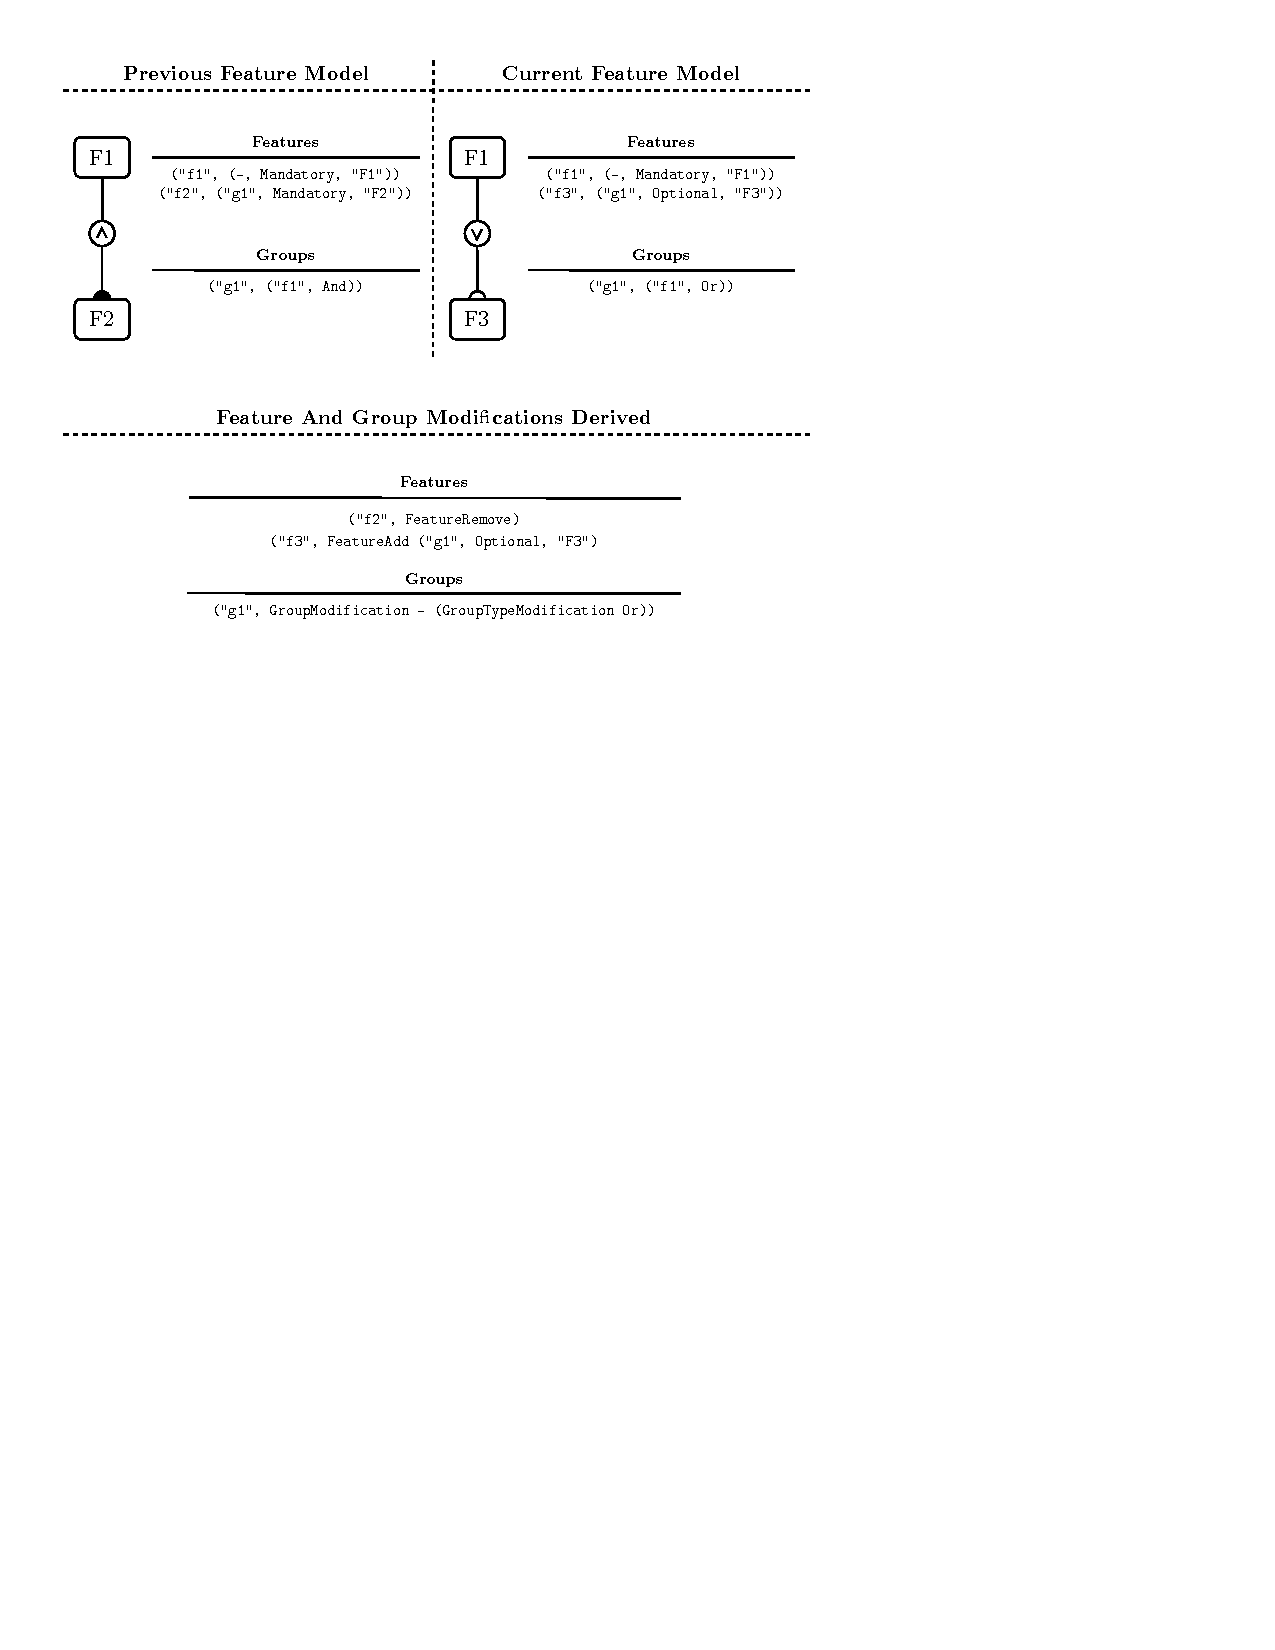
\includegraphics[]{feature_model_diff_visualized.pdf}
  \caption{A visualization of the result of running \texttt{diffFeatureModels} on two feature models}%
  \label{fig:diff_feature_models_visualized}
\end{figure}

In this example, we can see that the feature with id \texttt{f1} was unchanged, \texttt{f2} got removed and \texttt{f3} was added. As for our only group, \texttt{g1}, the type field of the group changed from \texttt{And} to \texttt{Or}. Although a bit simplified, the \texttt{merge} function will combine the features, \texttt{prev} and \texttt{curr} in the following way:

\begin{minted}[breaklines]{haskell}
prev   = [("f1", prevF1), ("f2", prevF2)]
curr   = [("f1", currF1),                 ("f3", currF3)]
result = [ ("f1", inBoth prevF1 currF1)
         , ("f2", inPrev prevF2)
         , ("f3", inNew currF3)
         ]
\end{minted}

Since both \texttt{prevF1} and \texttt{currF1} are equal, \texttt{inBoth} will return \texttt{Nothing}, representing that we don't need a modification. As for f2 and f3, \texttt{inPrev} and \texttt{inNew} will return \texttt{FeatureRemove} and \texttt{FeatureAdd} respectively.

\begin{minted}[breaklines]{haskell}
result = [ ("f1", Nothing)
         , ("f2", FeatureRemove)
         , ("f3", FeatureAdd ...)
         ]
\end{minted}

In the case of feature F1, since the feature appeared in both feature models, we are using the merge tactic \texttt{zipWithMaybeMatched}, which allows us to filter out results we do not want in the final mapping. Since we are not concerned about equal features, returning \texttt{Nothing} will tell the function to filter out the result.

The final result for our feature modification are the following:

\begin{minted}[breaklines]{haskell}
result = [("f2", FeatureRemove), ("f3", FeatureAdd ...)]
\end{minted}

As for our groups, we only have one, namely \texttt{g1}. Aligning and comparing our group results in the following:

\begin{minted}[breaklines]{haskell}
prev   = [("g1", prevGroup)]
curr   = [("g1", currGroup)]
result = [("g1", inBoth prevGroup currGroup)]
\end{minted}

Since the two groups are unequal, the result would be a \texttt{GroupModification} on the type field. By wrapping the modification in a \texttt{Just}, we are telling the merge tactic to include this result in the final mapping.

\begin{minted}[breaklines]{haskell}
result = [("g1", Just $ GroupModification Nothing 
                   (GroupTypeModification Or))]
\end{minted}

After applying the merge tactic \texttt{zipWithMaybeMatched}, we achieve our final result for the group modifications:

\begin{minted}[breaklines]{haskell}
result = [("g1", GroupModification Nothing 
                   (GroupTypeModification Or))]
\end{minted}

\section{Detecting the Changes Between Versions}%
\label{sec:detecting_the_changes_between_versions}

Up until this point, we have only considered transformations on single evolution plans. We have created a method of transforming a evolution plan into a merge-ready evolution plan using our two functions \texttt{flattenEvolutionPlan} and \texttt{deriveModifications}. However, since we want to merge two evolution plans into a single evolution plan, we have to figure out an approach to detecting, comparing and merging the changes into a single unified evolution plan.

The process of merging two different versions of an evolution plan involves figuring out what changes each version has made. In order to do so, we will utilize the common evolution plan both version were derived from, in order to confidently tell what changes has been made to each plan. As seen in our outline for the three-way merge algorithm in Figure~\vref{fig:merge_outline}, we will transform all three evolution plans into the \texttt{FlatModificationEvolutionPlan} representation, then attempt to merge version 1 and 2 with respect to the base evolution plan.

\subsection{A Simple Three-Way Merge Example}%
\label{sub:a_simple_three_way_merge_example}

Before we attempt to explain how the changes between the versions are detected and represented, we present a simple example consisting of three evolution plans. To create this merge example, we will revisit our simple evolution plan example visualized in Figure~\ref{fig:simpleep_treeuser}. The simple evolution plan presented will act as our base evolution plan. Using the base evolution plan, we will create two evolution plans, version 1 and version 2, which is derived from the common evolution plan. The changes to the derived evolution plans include the following:

\begin{itemize}
  \item \textbf{Version 1}: Includes two changes to the base evolution plan: (1) Adding a feature \texttt{F4} to the and-group at time point 1. (2) At time point 2, there was originally scheduled a group type modification from \texttt{And} to \texttt{Or}, but this version changed the modification to create a \texttt{Alternative} group instead.
  \item \textbf{Version 2}: Includes only one change to the base evolution plan. At time point 2, there was originally scheduled a renaming of the root feature. However, in this version, the scheduled renaming was removed.
\end{itemize}

The three evolution plans is visualized in Figure~\ref{fig:simple_three_way_example}. 

\begin{figure}[htpb]
  \centering
  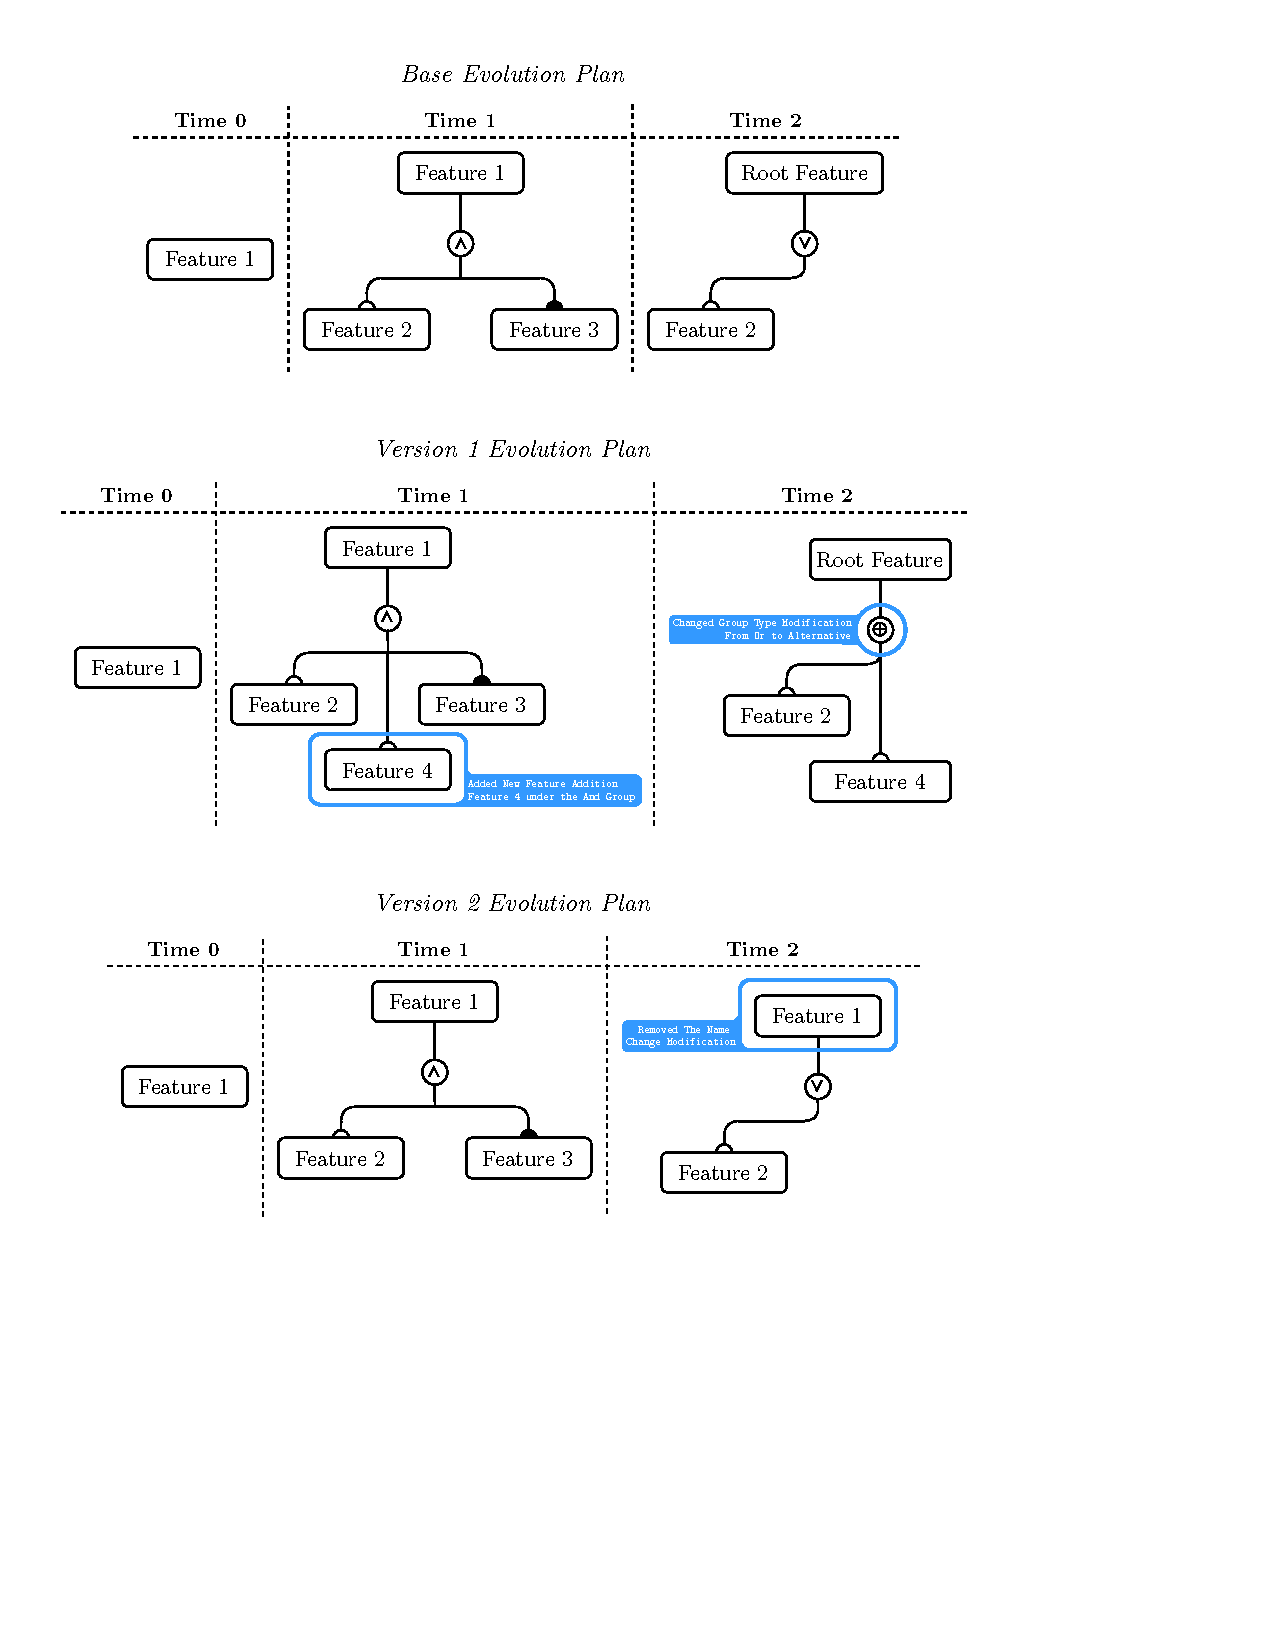
\includegraphics[width=\linewidth]{simple_three_way_example.pdf}
  \caption{A simple example of three evolution plans, as input of the three-way merge algorithm}%
  \label{fig:simple_three_way_example}
\end{figure}

\subsection{Representing Changes Between Versions}%
\label{sub:representing_changes_between_versions}

Before attempting to merge the different versions, we want to detect what \textit{changes} has been made in both derived versions. We present data types for representing such changes.

An important aspect to notice is the difference between \textit{modifications} and \textit{changes}. With modifications, we are talking about the changes between two feature models. The modifications are a part of the evolution plan, and has nothing to do with detecting changes between different versions. However, changes represent the actual changes that has been done to the base evolution plan in one of the derived versions.

With our changes, we are not adding, removing or changing features and groups, but rather adding, removing or changing the modifications themselves. The changes are working on a meta-level, allowing us to represent changes to the modifications. This distinction is a subtle, yet important factor. If one of the derived versions are removing a feature in a time point, this is actually represented as an addition. This is because the feature removal is represented as a new modification in the evolution plan, and we represent this by saying we "add" a new modification, which is the feature removal.

We present an evolution plan representing the merging of all three evolution plans. This representation follow a similar structure to our \texttt{FlatModificationEvolutionPlan}, which is why we reuse the data type \texttt{TransformationEvolutionPlan} defined in Section~\vref{sub:evolution_plan_definition_modification_level_flat_representation}.

\begin{minted}[breaklines]{haskell}
type MergeEvolutionPlan featureModel = 
  TransformationEvolutionPlan DiffResult featureModel
\end{minted}

The transformations between each time points are no longer represented as \texttt{Modifications}, but rather \texttt{DiffResult}. This data type represents the union of all the modifications from all three versions, sorted and organized to our needs. Each single feature and group modification are merged based on their id. The result of merging the three different modifications for a single feature or group is represented in \texttt{SingleDiffResult}, which can have three different outcomes:

\begin{itemize}
  \item \textbf{NoChange}: A modification existed in the base version, and was not changed or removed in either version.
  \item \textbf{ChangedInOne}: A modification \textit{changed} in one of the derived versions. This includes three scenarios; (1) a modification did not exist in the base, and were added in the derived version, (2) a modification existed in the base, but were removed in the derived version, and (3) a modification from the base were changed to another modification in the derived.
  \item \textbf{ChangedInBoth}: A modification changed in both versions. Similar to \texttt{ChangedInOne}, this includes changes where a modification existed in base and modifications where it did not exist.
\end{itemize}

The data types related to \texttt{DiffResult} are as follows:

\begin{minted}[breaklines]{haskell}
data DiffResult = DiffResult
  { features :: Map FeatureId FeatureDiffResult
  , groups :: Map GroupId GroupDiffResult
  }

type FeatureDiffResult =
  SingleDiffResult FeatureModification

type GroupDiffResult =
  SingleDiffResult GroupModification

-- Every possible combination that a feature
-- or group change could be modified
data SingleDiffResult modificationType
  = NoChange modificationType
  | ChangedInOne Version (OneChange modificationType)
  | ChangedInBoth (BothChange modificationType)

data OneChange modificationType
  = OneChangeWithBase
      modificationType -- Base
      (RemovedOrChangedModification modificationType)
        -- ^ Derived (V1 or V2)
  | OneChangeWithoutBase
      (AddedModification modificationType) 
        -- ^ Derived (V1 or V2)

data BothChange modificationType
  = BothChangeWithBase
      modificationType -- Base
      (RemovedOrChangedModification modificationType) -- V1
      (RemovedOrChangedModification modificationType) -- V2
  | BothChangeWithoutBase
      (AddedModification modificationType) -- V1
      (AddedModification modificationType) -- V2

data RemovedOrChangedModification modificationType
  = RemovedModification
  | ChangedModification modificationType

data AddedModification modificationType
  = AddedModification modificationType

data Version
  = V1
  | V2
\end{minted}

\subsubsection{Representing the changes from the example}%
\label{ssub:representing_the_changes_from_the_example}

Revisiting our example from Figure~\ref{fig:simple_three_way_example}, we can now represent the changes with our newly defined data types. Our merged version of the evolution plan is as follows:

\begin{minted}[breaklines]{haskell}
simpleExampleMergedPlan :: MergeEvolutionPlan FlatFeatureModel
simpleExampleMergedPlan =
  TransformationEvolutionPlan
    0
    initial
    [Plan 1 diffResult1, Plan 2 diffResult2]
  where
    initial =
      FlatFeatureModel
        "rootFeature"
        [
          ( "rootFeature"
          , FlatFeature Nothing Mandatory "Feature 1"
          )
        ]
        []
    diffResult1 =
      DiffResult
        [ ("feature2", NoChange 
            (FeatureAdd "group" Optional "Feature 2"))
        , ("feature3", NoChange
            (FeatureAdd "group" Mandatory "Feature 3"))
        , ("feature4", ChangedInOne V1 (OneChangeWithoutBase 
            (AddedModification 
              (FeatureAdd "group" Optional "Feature 4"))))
        ]
        [("group", NoChange 
           (GroupAdd "rootFeature" And))]
    diffResult2 =
      DiffResult
        [ ("feature3", NoChange FeatureRemove)
        , ("rootFeature", ChangedInOne V2 (OneChangeWithBase 
            (FeatureModification Nothing Nothing 
              (Just (FeatureNameModification "Root Feature"))) 
            RemovedModification))
        ]
        [ ("group", ChangedInOne V1 (OneChangeWithBase 
            (GroupModification Nothing 
              (Just (GroupTypeModification Or))) 
            (ChangedModification (GroupModification Nothing 
              (Just (GroupTypeModification Alternative))))))
        ]
\end{minted}

Since most of the modification remained unchanged, they are represented on the form \texttt{("id", NoChange modification)}. However, for our two changes in version 1, and one change in version 2, the changes are represented as \texttt{("id", ChangedInOne version change)}. Since we have no overlapping changes in the derived versions, we have no \texttt{ChangedInBoth} changes.

\subsection{Calculating the Changes}%
\label{sub:calculating_the_changes}

In order to merge the three three evolution plans into a evolution plan representing all the changes from the different versions, we define a function \texttt{createMergePlan}. Creating this representation requires unifying every time point in all three evolution plans. For each time point, the different modifications are combined into our new representation \texttt{DiffResult}. 

\begin{minted}[breaklines]{haskell}
createMergePlan ::
  FlatModificationEvolutionPlan ->
  FlatModificationEvolutionPlan ->
  FlatModificationEvolutionPlan ->
  MergeEvolutionPlan FlatFeatureModel
createMergePlan base v1 v2 =
  base & L.plans
    %~ \basePlans ->
      mergePlans
        basePlans
        (v1 ^. L.plans)
        (v2 ^. L.plans)

mergePlans ::
  [Plan Modifications] ->
  [Plan Modifications] ->
  [Plan Modifications] ->
  [Plan DiffResult]
mergePlans basePlans v1Plans v2Plans =
  mergePlansWithTimes
    (collectAllTimePoints basePlans v1Plans v2Plans)
    basePlans
    v1Plans
    v2Plans

mergePlansWithTimes ::
  [Time] ->
  [Plan Modifications] ->
  [Plan Modifications] ->
  [Plan Modifications] ->
  [Plan DiffResult]
mergePlansWithTimes [] _ _ _ = []
mergePlansWithTimes (time : times) basePlans v1Plans v2Plans =
  Plan
    time
    ( diffModifications
        baseModifications
        v1Modifications
        v2Modifications
    ) :
  mergePlansWithTimes
    times
    nextBasePlans
    nextV1Plans
    nextV2Plans
  where
    (baseModifications, nextBasePlans) =
      getModificationForTime basePlans time
    (v1Modifications, nextV1Plans) =
      getModificationForTime v1Plans time
    (v2Modifications, nextV2Plans) =
      getModificationForTime v2Plans time
\end{minted}

In some cases, one of the versions might introduce new time points. The new time points might be added at the end of the base evolution plan, and some times added somewhere in the middle of the existing plan. To handle this we define a function, \texttt{collectAllTimePoints}, for combining and collecting the time points for all the plans. We create \texttt{getModificationForTime}, which returns the modifications for a given time. Since the different plans doesn't necessarily include all the same time points, the function will create an empty list of modifications when a time point isn't present in the given evolution plan.

\begin{minted}[breaklines]{haskell}
collectAllTimePoints ::
  [Plan a] ->
  [Plan a] ->
  [Plan a] ->
  [Time]
collectAllTimePoints basePlans v1Plans v2Plans =
  merge (merge baseTimes v1Times) v2Times
  where
    baseTimes = basePlans ^.. traversed . L.timePoint
    v1Times = v1Plans ^.. traversed . L.timePoint
    v2Times = v2Plans ^.. traversed . L.timePoint
    merge (x : xs) (y : ys)
      | x == y = x : merge xs ys
      | x < y = x : merge xs (y : ys)
      | otherwise = y : merge (x : xs) ys
    merge xs ys = xs ++ ys

getModificationForTime ::
  [Plan Modifications] ->
  Time ->
  (Modifications, [Plan Modifications])
getModificationForTime [] _ = (emptyModifications, [])
getModificationForTime plans time =
  let Plan planTime modification : rest = plans
   in if time == planTime
        then (modification, rest)
        else (emptyModifications, plans)

emptyModifications :: Modifications
emptyModifications = Modifications M.empty M.empty
\end{minted}

The \texttt{diffModifications} function defined below will handle the transformation combining modifications into the \texttt{DiffResult} type. Combining the modifications of groups follow the same general process as with feature modifications. 

Combining the different \texttt{Map}s follow a similar approach as we did deriving the modifications between feature models (See Section~\vref{sub:the_final_merge_ready_representation}), using the \texttt{merge} function from \texttt{Data.Map.Merge}\footnote{https://hackage.haskell.org/package/containers-0.6.2.1/docs/Data-Map-Merge-Strict.html}. Since we are merging three maps instead of two, we combine the three maps in two steps; (1) We combine the two derived modifications into a intermediate result using the function \texttt{mergeDerived}, and (2), we combine the base modifications with the combined derived result using \texttt{mergeBaseAndDerived}.

\begin{minted}[breaklines]{haskell}
diffModifications ::
  Modifications ->
  Modifications ->
  Modifications ->
  DiffResult
diffModifications base v1 v2 =
  DiffResult
    ( mergeMaps
        (base ^. L.features)
        (v1 ^. L.features)
        (v2 ^. L.features)
    )
    ( mergeMaps
        (base ^. L.groups)
        (v1 ^. L.groups)
        (v2 ^. L.groups)
    )
  where
    mergeMaps baseMap v1Map v2Map =
      mergeBaseAndDerived
        baseMap
        $ mergeDerived v1Map v2Map

mergeBaseAndDerived ::
  (Ord a, Eq modification) =>
  M.Map a modification ->
  M.Map a (DerivedComparisionResult modification) ->
  M.Map a (SingleDiffResult modification)
mergeBaseAndDerived =
  Merge.merge
    (Merge.mapMissing (const inBase))
    (Merge.mapMissing (const inDerived))
    (Merge.zipWithMatched (const inBoth))
  where
    inBase baseMod = withBase baseMod Nothing Nothing
    inDerived derivedResult =
      case derivedResult of
        OneVersion version mod ->
          ChangedInOne
            version
            (OneChangeWithoutBase (AddedModification mod))
        BothVersions v1Mod v2Mod ->
          ChangedInBoth
            ( BothChangeWithoutBase
                (AddedModification v1Mod)
                (AddedModification v2Mod)
            )
    inBoth baseMod derivedResult =
      case derivedResult of
        OneVersion V1 mod ->
          withBase baseMod (Just mod) Nothing
        OneVersion V2 mod ->
          withBase baseMod Nothing (Just mod)
        BothVersions v1Mod v2Mod ->
          withBase baseMod (Just v1Mod) (Just v2Mod)
    withBase baseMod mV1Mod mV2Mod =
      case (Just baseMod /= mV1Mod, Just baseMod /= mV2Mod) of
        (True, True) ->
          ChangedInBoth
            ( BothChangeWithBase
                baseMod
                (removeOrChanged mV1Mod)
                (removeOrChanged mV2Mod)
            )
        (True, False) ->
          ChangedInOne
            V1
            ( OneChangeWithBase
                baseMod
                (removeOrChanged mV1Mod)
            )
        (False, True) ->
          ChangedInOne
            V2
            ( OneChangeWithBase
                baseMod
                (removeOrChanged mV2Mod)
            )
        (False, False) -> NoChange baseMod
    removeOrChanged Nothing = RemovedModification
    removeOrChanged (Just mod) = ChangedModification mod

data DerivedComparisionResult modification
  = OneVersion Version modification
  | BothVersions modification modification

mergeDerived ::
  Ord a =>
  M.Map a modification ->
  M.Map a modification ->
  M.Map a (DerivedComparisionResult modification)
mergeDerived =
  Merge.merge
    (Merge.mapMissing (const (OneVersion V1)))
    (Merge.mapMissing (const (OneVersion V2)))
    (Merge.zipWithMatched (const BothVersions))
\end{minted}

\section{Merging Intended Changes}%
\label{sec:merging_intended_changes}

Now that we have a representation for the unification off all three evolution plans, we can begin the process of creating a single merged evolution plan. We created the type \texttt{MergeEvolutionPlan} for having a representation for all three evolution plans, and our \texttt{createMergePlan} for transforming the three evolution plans to this representation. We will now present the next step of our algorithm, \texttt{unifyMergePlan}, which joins the different modifications in the \texttt{MergeEvolutionPlan} and produces a single, unified \texttt{FlatModificationEvolutionPlan}.

We can notice from the three-way merge algorithm outline from Figure~\vref{fig:merge_outline} that the \texttt{mergePlan} was split into two parts, \texttt{createMergePlan} and \texttt{unifyMergePlan}. This had several benefits. Both functions had clearly defined purposes. The only purpose of \texttt{createMergePlan} was to create a better representation for all the modifications, making it easier to see what changes each version made to the base. Having an intermediate representation like \texttt{MergeEvolutionPlan} also serves as documentation, letting the reader see more clearly what cases has to be considered. This benefit is also present in our \texttt{unifyMergePlan} algorithm defined below, since we now can see what modification the algorithm chooses, which it discards, and which combinations result in errors.

\subsection{Merge Conflicts}%
\label{sub:merge_errors}

In our three-way merge algorithm, unifying the merge plan is our first point of potential failure. As mentioned in the section discussing conflicts (Section~\vref{sub:conflicts}), merging the efforts into a single evolution plan might result in \textit{merge} conflicts. A merge conflict could arise due to diverging changes for a single feature or group. This can only happen when a change is present in both derived versions. Modeling our potential conflicts are done in the following way:

\begin{minted}[breaklines]{haskell}
data Conflict
  = Merge Time MergeConflict
  | Local Time LocalConflict
  | Global Time GlobalConflict
\end{minted}

All of our different conflict types store the time in which the error occured, as well as information specific to the given conflict. Since merging the plan could only raise a merge conflict, we will get in to the detail of local and global conflicts later. We define \texttt{MergeConflict} as follows:

\begin{minted}[breaklines]{haskell}
data MergeConflict
  = FeatureConflict FeatureId (BothChange FeatureModification)
  | GroupConflict GroupId (BothChange GroupModification)
\end{minted}

Notice that we reuse the \texttt{BothChange} from our definition of \texttt{MergeEvolutionPlan}. This contains all information about what modification was originally in the base evolution plan, as well as what change were made in both versions.

\subsubsection{Propagating the errors}%
\label{ssub:propagating_the_errors}

As we will see in the definitions below, the \texttt{unifyMergePlan} algorithm takes our \texttt{MergeEvolutionPlan} as an argument, and returns an \texttt{Either Conflict FlatModificationEvolutionPlan}. Returning an \texttt{Either} means that the algorithm will either succeed, which will yield a \texttt{Right flatModEP}, or it will fail, yielding a \texttt{Left conflict}. The function will attempt to unify every time point, change and modification into our \texttt{FlatModificationEvolutionPlan}. If it produces a merge conflict somewhere, the conflict would automatically propagate upwards until the entire merge algorithm results in a conflict.

To achieve this without to much bloat, we will leverage Haskell's powerful type system and syntactic abstractions. Using functions such as \texttt{\%\%\~} and \texttt{M.traverseMaybeWithKey}, as well as syntactic abstractions like \texttt{do}-notation, we can let the conflicts and errors automatically propagate once they occur. We will not go into great detail about how this works, but it is beneficial to know that once a conflict occurs, the conflict is propagated to the top level.

\subsection{Specifying the Unification of the Merge Plan}%
\label{sub:specifying_the_unification_of_the_merge_plan}

The first three functions will look at the plans for each time point. Each time point contains information about the modifications of features and groups, as well as how each derived version changed these modifications. The functions will go through each feature and group, and call the \texttt{unifySingleDiffResult} to unify the changes to a single feature or group.

\begin{minted}[breaklines]{haskell}
unifyMergePlan ::
  MergeEvolutionPlan FlatFeatureModel ->
  Either Conflict FlatModificationEvolutionPlan
unifyMergePlan =
  L.plans . traversed %%~ unifyTimePointResult

unifyTimePointResult ::
  Plan DiffResult ->
  Either Conflict (Plan Modifications)
unifyTimePointResult (Plan time (DiffResult fs gs)) = do
  fs' <- unifyModificationsMap FeatureConflict time fs
  gs' <- unifyModificationsMap GroupConflict time gs
  return $ Plan time (Modifications fs' gs')

unifyModificationsMap ::
  Eq modificationType =>
  (modIdType -> BothChange modType -> MergeConflict) ->
  Time ->
  M.Map modIdType (SingleDiffResult modType) ->
  Either Conflict (M.Map modIdType modType)
unifyModificationsMap checkBothOverlapping timePoint =
  M.traverseMaybeWithKey
    (unifySingleDiffResult checkBothOverlapping timePoint)
\end{minted}

The main work is done converting a \texttt{SingleDiffResult} to a \texttt{modificationType}. This function is general and works for both features and groups, meaning we will get either a \texttt{FeatureModification} or a \texttt{GroupModification}. This function will fail with a conflict if two changes from the derived versions cannot be unified. If it succeeds, the function can either return \texttt{Nothing}, indicating that an modification were removed and should not occur in the merged evolution plan, or we return \texttt{Just modification} if a modification should occur in the merged plan.

\begin{minted}[breaklines]{haskell}
unifySingleDiffResult ::
  Eq modType =>
  (modIdType -> BothChange modType -> MergeConflict) ->
  Time ->
  modIdType ->
  SingleDiffResult modType ->
  Either Conflict (Maybe modType)
unifySingleDiffResult conflictHandler time id diffResult =
  case diffResult of
    NoChange baseMod ->
      Right (Just baseMod)
    ChangedInOne version (OneChangeWithBase baseMod RemovedModification) ->
      Right Nothing
    ChangedInOne version (OneChangeWithBase baseMod (ChangedModification derivedMod)) ->
      Right (Just derivedMod)
    ChangedInOne version (OneChangeWithoutBase (AddedModification derivedMod)) ->
      Right (Just derivedMod)
    ChangedInBoth bothChange ->
      checkOverlappingChanges
        conflictHandler
        time
        id
        bothChange
\end{minted}

In case both versions changed a feature or group modification, we only want to raise an error if the changes were different.

\begin{minted}[breaklines]{haskell}
checkOverlappingChanges ::
  Eq modType =>
  (modIdType -> BothChange modType -> MergeConflict) ->
  Time ->
  modIdType ->
  BothChange modType ->
  Either Conflict (Maybe modType)
checkOverlappingChanges conflictHandler time id bothChange =
  case bothChange of
    BothChangeWithoutBase (AddedModification v1) (AddedModification v2) ->
      ensureNotConflicting v1 v2
    BothChangeWithBase base RemovedModification RemovedModification ->
      Right Nothing
    BothChangeWithBase base (ChangedModification v1) (ChangedModification v2) ->
      ensureNotConflicting v1 v2
    BothChangeWithBase{} ->
      conflict
  where
    conflict = Left (Merge time (conflictHandler id bothChange))
    ensureNotConflicting v1Modification v2Modification =
      if v1Modification == v2Modification
        then Right (Just v1Modification)
        else conflict
\end{minted}

\subsection{Example}%
\label{sub:example_unified_merge}

Looking at our running example, visualized in Figure~\vref{fig:simple_three_way_example}, the result of merging the three plans is successful. Since none of the changes from each version overlap, no merge conflict was produced either. Each change in both versions was included, and the result was the following:

\begin{minted}[breaklines]{haskell}
simpleExampleUnifiedPlan 
  :: Either Conflict FlatModificationEvolutionPlan
simpleExampleUnifiedPlan =
  Right $
    TransformationEvolutionPlan
      0
      initial
      [ Plan 1 modifications1
      , Plan 2 modifications2
      ]
  where
    initial =
      FlatFeatureModel
        "rootFeature"
        [
          ( "rootFeature"
          , FlatFeature Nothing Mandatory "Feature 1"
          )
        ]
        []
    modifications1 =
      Modifications
        [
          ( "feature2"
          , FeatureAdd "group" Optional "Feature 2"
          )
        ,
          ( "feature3"
          , FeatureAdd "group" Mandatory "Feature 3"
          )
        ,
          ( "feature4"
          , FeatureAdd "group" Optional "Feature 4"
          )
        ]
        [("group", GroupAdd "rootFeature" And)]
    modifications2 =
      Modifications
        [("feature3", FeatureRemove)]
        [
          ( "group"
          , GroupModification
              Nothing
              (Just (GroupTypeModification Alternative))
          )
        ]
\end{minted}

The result of the \texttt{unifyMergePlan} function returned what we wanted. From both derived versions, there was a total of three changes. A new feature was added at time 1, the name change in time 2 was removed and the group type modification in time 2 was changed to transform to a \texttt{Alternative} group instead of \texttt{Or} group.

\section{Ensuring structural and semantic soundness}%
\label{sec:ensuring_structural_and_semantic_soundness_of_merge_result}

Now that we have defined a method of detecting and merging changes to evolution plans, we would have to check that the resulting evolution plan results in a valid and sound evolution plan, keeping both the structure and semantics in tact.

To ensure soundness, we will design an algorithm that makes sure that each modification is valid. In order to do so, we will convert our \texttt{FlatModificationEvolutionPlan} representation back to our normal form for evolution plans, namely \texttt{TreeUserEvolutionPlan}. Doing so will let us see the effects of applying each modification, and ensuring the resulting feature models and evolution plan is correct.

Looking back at the algorithm outline in Figure~\vref{fig:merge_outline}, we can see that there are three remaining steps in the algorithm; \texttt{integrateModifications}, \texttt{checkModifications} and \texttt{unflattenEvolutionPlan}. First, we will take the unchecked evolution plan and integrate every modification for each time point. Next, we will check that the resulting feature models are following the structural and semantic constraints of evolution plans. Lastly, we will convert the sound evolution plan back to our tree-based normal form for evolution plans. Each of these steps are discussed in more detail in Section~\ref{sub:applying_modifications}, Section~\ref{sub:checking_dependencies_and_ensuring_soundness} and Section~\ref{sub:converting_back_to_normal_form}. 

\paragraph{Integrating and Checking Modifications}%
\label{par:integrating_and_checking_modifications}

In reality, the two steps \texttt{integrateModifications} and \texttt{checkModifications} are more tightly integrated than visualized in the outline. Instead, we have a single algorithm for doing both things, \texttt{integrateAndCheckModifications}. By starting with the initial feature model and the first time point, the function will first apply every modification to the feature model, then check that the result is sound. With the resulting feature model, we will take the next time point and do the process all over again. This will continue until we have a list of feature models that are checked for soundness.

For a single time point, we need to apply all the modifications before checking for soundness. This is due to us having no specific ordering of operations, and the feature model might be temporarily invalid while applying modifications. For this reason, we will not check constrains immediately after applying a modification. Instead, we will note the potential points where our result might be invalid, and check those after every modification has been integrated at a certain time.

When applying modifications, we generate a list of \textit{dependencies} that we will later pass onto \texttt{checkModifications}. What dependencies arise will depend on the modification at hand, but typically these dependencies include things like checking for cycles, non-existing parent relations or well-formedness constraints. These dependencies along with the current feature model are then passed onto \texttt{checkModifications}, which will check every dependency and either accept or reject the feature model.

Below, we will define the code necessary to intertwine both the integration and soundness checking of modifications. Since integrating and checking modifications both can lead to conflicts, the functions will return \texttt{Either Conflict value} instead of just \texttt{value}. Using do-notation, the monadic structure will make sure the error is propagated immediately if a conflict occurs.

\begin{minted}[breaklines]{haskell}
integrateAndCheckModifications ::
  FlatModificationEvolutionPlan ->
  Either Conflict FlatUserEvolutionPlan
integrateAndCheckModifications evolutionPlan =
  case evolutionPlan of
    TransformationEvolutionPlan initialTime initialFM plans ->
      UserEvolutionPlan
        <$> scanEvolutionPlan
          plans
          (TimePoint initialTime initialFM)

scanEvolutionPlan ::
  [Plan Modifications] ->
  TimePoint FlatFeatureModel ->
  Either Conflict [TimePoint FlatFeatureModel]
scanEvolutionPlan [] timePoint = return [timePoint]
scanEvolutionPlan (plan : plans) currentTimePoint = do
  (nextTimePointUnchecked, dependencies) <-
    runWriterT $ integrateSinglePlan plan currentTimePoint
  nextTimePoint <-
    checkGlobalConflict dependencies nextTimePointUnchecked
  convertedEvolutionPlan <-
    scanEvolutionPlan plans nextTimePoint
  return $ currentTimePoint : convertedEvolutionPlan
\end{minted}

As discussed, the first part is integrating the modifications. Most of the work is here done by \texttt{integrateSinglePlan}, which returns a \texttt{WriterT [Dependency] (Either Conflict) (TimePoint FlatFeatureModel)}. Using the \texttt{Writer} and \texttt{Either} monad, we can write a function that handles conflicts, writing dependencies and returning the merged time point without to much boilerplate. This is made possible by the \texttt{WriterT} monad transformer, which allows us to compose monads. In this case, we have our \texttt{Either Conflict} monad, which lets us propagate errors. As we integrate modifications one by one, we also generate a list of dependencies, which the \texttt{Writer} monad lets us do without much boilerplate. These two monads are then combined, allowing us to use the \texttt{runWriterT} functions which returns both the next time point as well as the dependencies that needs to be checked in an \texttt{Either} environment that propagates errors when they occur.

The generated dependencies and the next time point are then passed to \texttt{checkGlobalConflict}, which either succeeds or raise a conflict. Upon failure, the do-notation and monadic structure will propagate the error. However, if it succeeds, the rest of the time points are recursively called.

\subsection{Applying modifications}%
\label{sub:applying_modifications}

In order to integrate every single modifications for a single time point, the \texttt{integrateSinglePlan} function is called. As discussed, the modifications for a single time point has no ordering, so we can arbitrarily choose an application ordering. The modifications are applied by calling either \texttt{integrateFeature} or \texttt{integrateGroup} with the feature model, which will return the feature model with the modification applied. The resulting feature model is then passed to the next modification. The process is continued until all modifications are applied.

The core idea of this is the \texttt{foldl} function, which has the following signature for lists: \texttt{(fm -> mod -> fm) -> fm -> [mod] -> fm}. Using it for our purpose, it will apply the modifications on the feature model as discussed. However, we will use the more complicated variant, \texttt{ifoldlMOf} instead. The main reason is that it allows us to fold in a monadic context. In our instance, our monad is both the \texttt{Writer} and \texttt{Either} monad. This means that if an error occurs somewhere, the computation will stop and the conflict will be returned. The \texttt{Writer} monad lets us append dependencies without actually worrying about passing the list of dependencies as argument and returning it from the functions.

\begin{minted}[breaklines]{haskell}
integrateSinglePlan ::
  Plan Modifications ->
  TimePoint FlatFeatureModel ->
  WriterT
    [Dependency]
    (Either Conflict)
    (TimePoint FlatFeatureModel)
integrateSinglePlan
  (Plan nextTime modifications)
  (TimePoint _ featureModel) =
    TimePoint nextTime <$> newFeatureModel
    where
      newFeatureModel =
        integrateFeatures featureModel >>= integrateGroups
      integrateFeatures fm =
        ifoldlMOf
          (L.features . itraversed)
          (integrateFeature nextTime)
          fm
          modifications
      integrateGroups fm =
        ifoldlMOf
          (L.groups . itraversed)
          (integrateGroup nextTime)
          fm
          modifications
\end{minted}

The \texttt{integrateFeature} and \texttt{integrateGroup} functions will be given a modification on a feature or group, as well as the current feature model. Based on the type of modification, the function will write dependencies with the \texttt{tell} function as well as incorporate the modification in the feature model. If a conflict occurs somewhere, the \texttt{throwError} function will be used to short circuit the function and return the conflict to the top level.

\begin{minted}[breaklines]{haskell}
integrateFeature ::
  Time ->
  FeatureId ->
  FlatFeatureModel ->
  FeatureModification ->
  WriterT [Dependency] (Either Conflict) FlatFeatureModel
integrateFeature time featureId fm featureMod =
  case featureMod of
    FeatureAdd parentGroupId featureType name ->
      case M.lookup featureId (fm ^. L.features) of
        Nothing -> do
          tell
            . fmap (FeatureDependency featureMod)
            $ [ ParentGroupExists parentGroupId
              , UniqueName name
              , FeatureIsWellFormed featureId
              ]
          return $
            fm
              & L.features
                . at featureId
                ?~ FlatFeature
                  (Just parentGroupId)
                  featureType
                  name
        Just oldFeature ->
          throwError $
            Local
              time
              (FeatureAlreadyExists featureMod featureId)
    FeatureRemove ->
      case M.lookup featureId (fm ^. L.features) of
        Nothing ->
          throwError $
            Local
              time
              (FeatureNotExists featureMod featureId)
        Just oldFeature -> do
          tell . fmap (FeatureDependency featureMod) $
            [NoChildGroups featureId]
          return $ fm & L.features . at featureId .~ Nothing
    FeatureModification parentIdMod featureTypeMod nameMod ->
      if has (L.features . ix featureId) fm
        then
          pure fm
            >>= integrateParentMod
            >>= integrateTypeMod
            >>= integrateNameMod
        else
          throwError $
            Local time (FeatureNotExists featureMod featureId)
      where
        integrateParentMod ::
          FlatFeatureModel ->
          WriterT
            [Dependency]
            (Either Conflict)
            FlatFeatureModel
        integrateParentMod fm =
          case parentIdMod of
            Nothing -> return fm
            Just (FeatureParentModification newValue) -> do
              tell . fmap (FeatureDependency featureMod) $
                [ ParentGroupExists newValue
                , NoCycleFromFeature featureId
                , FeatureIsWellFormed featureId
                ]
              return $
                fm
                  & L.features
                    . ix featureId
                    . L.parentGroupId
                    ?~ newValue

        integrateTypeMod ::
          FlatFeatureModel ->
          WriterT
            [Dependency]
            (Either Conflict)
            FlatFeatureModel
        integrateTypeMod fm =
          case featureTypeMod of
            Nothing -> return fm
            Just (FeatureTypeModification newValue) -> do
              tell . fmap (FeatureDependency featureMod) $
                [FeatureIsWellFormed featureId]
              return $
                fm
                  & L.features
                    . ix featureId
                    . L.featureType
                  .~ newValue

        integrateNameMod ::
          FlatFeatureModel ->
          WriterT
            [Dependency]
            (Either Conflict)
            FlatFeatureModel
        integrateNameMod fm =
          case nameMod of
            Nothing -> return fm
            Just (FeatureNameModification newValue) -> do
              tell . fmap (FeatureDependency featureMod) $
                [UniqueName newValue]
              return $
                fm
                  & L.features
                    . ix featureId
                    . L.name
                  .~ newValue

integrateGroup ::
  Time ->
  GroupId ->
  FlatFeatureModel ->
  GroupModification ->
  WriterT [Dependency] (Either Conflict) FlatFeatureModel
integrateGroup time groupId fm groupMod =
  case groupMod of
    GroupAdd parentFeatureId groupType ->
      case M.lookup groupId (fm ^. L.groups) of
        Nothing -> do
          tell . fmap (GroupDependency groupMod) $
            [ ParentFeatureExists parentFeatureId
            ]
          return $
            fm
              & L.groups
                . at groupId
                ?~ FlatGroup parentFeatureId groupType
        Just oldGroup ->
          throwError $
            Local
              time
              (GroupAlreadyExists groupMod groupId)
    GroupRemove ->
      case M.lookup groupId (fm ^. L.groups) of
        Nothing ->
          throwError $
            Local
              time
              (GroupNotExists groupMod groupId)
        Just oldGroup -> do
          tell . fmap (GroupDependency groupMod) $
            [NoChildFeatures groupId]
          return $ fm & L.groups . at groupId .~ Nothing
    GroupModification parentFeatureIdMod groupTypeMod ->
      if has (L.groups . ix groupId) fm
        then
          pure fm
            >>= integrateParentMod
            >>= integrateTypeMod
        else
          throwError $
            Local time (GroupNotExists groupMod groupId)
      where
        integrateParentMod ::
          FlatFeatureModel ->
          WriterT
            [Dependency]
            (Either Conflict)
            FlatFeatureModel
        integrateParentMod fm =
          case parentFeatureIdMod of
            Nothing -> return fm
            Just (GroupParentModification newValue) -> do
              tell . fmap (GroupDependency groupMod) $
                [ ParentFeatureExists newValue
                , NoCycleFromGroup groupId
                ]
              return $
                fm
                  & L.groups
                    . ix groupId
                    . L.parentFeatureId
                  .~ newValue

        integrateTypeMod ::
          FlatFeatureModel ->
          WriterT
            [Dependency]
            (Either Conflict)
            FlatFeatureModel
        integrateTypeMod fm =
          case groupTypeMod of
            Nothing -> return fm
            Just (GroupTypeModification newValue) -> do
              tell . fmap (GroupDependency groupMod) $
                [GroupIsWellFormed groupId]
              return $
                fm
                  & L.groups
                    . ix groupId
                    . L.groupType
                  .~ newValue
\end{minted}

\subsection{Local Conflicts}%
\label{sub:local_conflicts}

As seen in the code above, the integration of modifications to the feature model can potentially lead to \textit{local} conflicts. When we try to integrate the set of modifications at a certain time point, we want to make sure the feature model after applying every modification is sound. This means that we allow for the feature model to be invalid while we are under the process of applying the modifications. However, some changes can be guaranteed to result in an unsound feature model.

Local conflicts occur when we try to alter or remove features or groups that don't exist, or when we try to add features that already exist. Since our modifications are modeled as maps with ids as keys, we guarantee that a feature or group only has a single modification. This implies that we can not add then remove a feature in the same time point. The local conflicts can thus be reported immediately without checking the rest of the modifications at the time point.

\begin{minted}[breaklines]{haskell}
data LocalConflict
  = FeatureAlreadyExists FeatureModification FeatureId
  | FeatureNotExists FeatureModification FeatureId
  | GroupAlreadyExists GroupModification GroupId
  | GroupNotExists GroupModification GroupId
\end{minted}

\subsection{Dependencies}%
\label{sub:dependencies}

With local conflicts, the conflicts were local to the single feature or group at hand. These conflicts could be raised without knowing what the rest of the modifications were. However, some of the modifications relied on knowing the state of other features or groups, which prevents us from reporting these conflicts immediately. Some modifications, i.e. adding a feature, relied on parent nodes to exist. However, to know if the parent existed or not, we would have to apply the rest of the modifications in case the parent also was removed or added. For this reason, we postpone the checking until after every modification has been included, generating dependencies which marks what we need to check. The different dependencies are defined below.

\begin{minted}[breaklines]{haskell}
data Dependency
  = FeatureDependency FeatureModification FeatureDependencyType
  | GroupDependency GroupModification GroupDependencyType

data FeatureDependencyType
  = NoChildGroups FeatureId
  | ParentGroupExists GroupId
  | NoCycleFromFeature FeatureId
  | FeatureIsWellFormed FeatureId
  | UniqueName String

data GroupDependencyType
  = NoChildFeatures GroupId
  | ParentFeatureExists FeatureId
  | NoCycleFromGroup GroupId
  | GroupIsWellFormed GroupId
\end{minted}

Each modification yields a set of dependencies depending on what conflicts could potentially rise. This is encoded in the \texttt{integrateFeature} and \texttt{integrateGroup} functions, as well as visualized in Table~\vref{tab:generated_dependencies}

\begin{table}[htpb]
  \centering
  \label{tab:generated_dependencies}
  \begin{tabular}{c|c}
    \textbf{Modification Type} & \textbf{Generated Dependencies} \\ \hline
    Add Feature & \begin{tabular}[c]{@{}c@{}}ParentGroupExists\\ UniqueName\\ FeatureIsWellFormed\end{tabular} \\ \hline
    Remove Feature & NoChildGroups \\ \hline
    Modify Feature Parent & \begin{tabular}[c]{@{}c@{}}ParentGroupExists\\ NoCycleFromFeature\\ FeatureIsWellFormed\end{tabular} \\ \hline
    Modify Feature Type & FeatureIsWellFormed \\ \hline
    Modify Feature Name & UniqueName \\ \hline
    Add Group & ParentFeatureExists \\ \hline
    Remove Group & NoChildFeatures \\ \hline
    Modify Group Parent & \begin{tabular}[c]{@{}c@{}}ParentFeatureExists\\ NoCycleFromGroup\end{tabular} \\ \hline
    Modify Group Type & GroupIsWellFormed
  \end{tabular}
  \caption{Generated dependencies}
\end{table}

\subsection{Global Conflicts}%
\label{sub:global_conflicts}

The last kind of conflicts we could encounter is the \textit{global} conflict. For a given time point, we generated a list of dependencies we needed to check. If one or more dependencies are not met, we raise a global conflict. This is done by collecting the failed dependencies and returning them as a list.

\begin{minted}[breaklines]{haskell}
data GlobalConflict
  = FailedDependencies [Dependency]
\end{minted}

\subsection{Checking dependencies and ensuring soundness}%
\label{sub:checking_dependencies_and_ensuring_soundness}

After applying every modification for a certain time point, the generated dependencies and resulting feature model are passed to the \texttt{checkGlobalConflict}. The function will either succeed with the correct feature model, or fail with a list of dependencies that did not pass.

\begin{minted}[breaklines]{haskell}
checkGlobalConflict ::
  [Dependency] ->
  TimePoint FlatFeatureModel ->
  Either Conflict (TimePoint FlatFeatureModel)
checkGlobalConflict dependencies tp =
  errorIfFailed (filter (not . checkDependency) dependencies)
  where
    TimePoint time featureModel = tp
    errorIfFailed failedDeps =
      case failedDeps of
        [] -> Right tp
        _ -> Left $ Global time (FailedDependencies failedDeps)
    checkDependency (FeatureDependency featureMod dType) =
      case dType of
        NoChildGroups featureId ->
          hasn't
            ( L.groups
                . traversed
                . L.parentFeatureId
                . filtered (== featureId)
            )
            featureModel
        ParentGroupExists groupId ->
          has
            (L.groups . ix groupId)
            featureModel
        NoCycleFromFeature featureId ->
          not $ featureInCycle S.empty featureId featureModel
        FeatureIsWellFormed featureId ->
          -- If mandatory feature, parent has to be AND group
          -- === feature not mandatory or parent is and
          let featureType =
                featureModel
                  ^?! L.features
                    . ix featureId
                    . L.featureType
              parentGroupType =
                featureModel
                  ^?! L.parentGroupOfFeature featureId
                    . L.groupType
           in featureType /= Mandatory
                || parentGroupType == And
        UniqueName name ->
          lengthOf
            ( L.features
                . traversed
                . L.name
                . filtered (== name)
            )
            featureModel
            <= 1
    checkDependency (GroupDependency groupMod dType) =
      case dType of
        NoChildFeatures groupId ->
          hasn't
            ( L.features
                . traversed
                . L.parentGroupId
                . filtered (== Just groupId)
            )
            featureModel
        ParentFeatureExists featureId ->
          has
            (L.features . ix featureId)
            featureModel
        NoCycleFromGroup groupId ->
          not $ groupInCycle S.empty groupId featureModel
        GroupIsWellFormed groupId ->
          -- Either the group is a AND group
          -- or all child features are optional
          let groupType =
                featureModel
                  ^?! L.groups
                    . ix groupId
                    . L.groupType
              childFeatureTypes =
                featureModel
                  ^.. L.childFeaturesOfGroup groupId
                    . L.featureType
           in groupType == And
                || all (== Optional) childFeatureTypes

featureInCycle ::
  S.Set (Either FeatureId GroupId) ->
  FeatureId ->
  FlatFeatureModel ->
  Bool
featureInCycle visited featureId featureModel
  | Left featureId `elem` visited = True
  | otherwise =
    case featureModel
      ^? L.features
        . ix featureId
        . L.parentGroupId
        . _Just of
      Nothing -> False -- no parent group/non existing feature
      Just parentGroupId ->
        groupInCycle
          (S.insert (Left featureId) visited)
          parentGroupId
          featureModel

groupInCycle ::
  S.Set (Either FeatureId GroupId) ->
  GroupId ->
  FlatFeatureModel ->
  Bool
groupInCycle visited groupId featureModel
  | Right groupId `elem` visited = True
  | otherwise =
    case featureModel
      ^? L.groups
        . ix groupId
        . L.parentFeatureId of
      Nothing -> False -- non existing group
      Just parentFeatureId ->
        featureInCycle
          (S.insert (Right groupId) visited)
          parentFeatureId
          featureModel
\end{minted}

\subsection{Converting Back to Normal Form}%
\label{sub:converting_back_to_normal_form}

The last steps of the three-way algorithm transformed the \texttt{FlatModificationEvolutionPlan} back to \texttt{FlatUserEvolutionPlan}, which models the evolution plan as a list of feature models. The final and last step of the algorithm is converting this back to the \texttt{TreeUserEvolutionPlan}, which models each feature model in a recursive tree-structure instead of the flat mapping based way.

This is done by retrieving the root feature and its child groups. The child groups are recursively transformed to our tree representation, and combined with the root feature to create our recursive tree structure.

\begin{minted}[breaklines]{haskell}
unflattenSoundEvolutionPlan ::
  FlatUserEvolutionPlan ->
  TreeUserEvolutionPlan
unflattenSoundEvolutionPlan =
  L.timePoints
    . traversed
    %~ unflattenTimePoint

unflattenTimePoint ::
  TimePoint FlatFeatureModel ->
  TimePoint TreeFeatureModel
unflattenTimePoint (TimePoint time featureModel) =
  TimePoint time $
    TreeFeatureModel $
      unflattenFeature featureModel (featureModel ^. L.rootId)

unflattenFeature ::
  FlatFeatureModel ->
  FeatureId ->
  TreeFeature
unflattenFeature featureModel featureId =
  TreeFeature featureId featureType name childGroups
  where
    childGroupIds =
      featureModel
        ^.. L.ichildGroupsOfFeature featureId . asIndex
    childGroups =
      S.fromList $
        fmap (unflattenGroup featureModel) childGroupIds
    (FlatFeature _ featureType name) =
      featureModel ^?! L.features . ix featureId

unflattenGroup ::
  FlatFeatureModel ->
  GroupId ->
  TreeGroup
unflattenGroup featureModel groupId =
  TreeGroup groupId groupType childFeatures
  where
    childFeatureIds =
      featureModel
        ^.. L.ichildFeaturesOfGroup groupId
          . asIndex
    childFeatures =
      S.fromList $
        fmap (unflattenFeature featureModel) childFeatureIds
    (FlatGroup _ groupType) =
      featureModel ^?! L.groups . ix groupId
\end{minted}

\subsection{Example}%
\label{sub:example}

\subsubsection{After Applying and Checking Modifications}%
\label{ssub:after_applying_and_checking_modifications}

Revisiting our simple example from Figure~\vref{fig:simple_three_way_example}, we pick up the example from where we left off. With the \texttt{FlatModificationEvolutionPlan} representation of the merged plan, we use \texttt{integrateAndCheckModifications} to apply the modifications and check the result for soundness. This results in a list of feature models, in our \texttt{FlatUserEvolutionPlan} representation. The result can be seen below.

\begin{minted}[breaklines]{haskell}
simpleExampleCheckedPlan :: 
  Either Conflict FlatUserEvolutionPlan
simpleExampleCheckedPlan =
  Right $
    UserEvolutionPlan
      [ TimePoint 0 fm0
      , TimePoint 1 fm1
      , TimePoint 2 fm2
      ]
  where
    fm0 =
      FlatFeatureModel
        "rootFeature"
        [
          ( "rootFeature"
          , FlatFeature
              Nothing
              Mandatory
              "Feature 1"
          )
        ]
        []
    fm1 =
      FlatFeatureModel
        "rootFeature"
        [
          ( "feature2"
          , FlatFeature
              (Just "group")
              Optional
              "Feature 2"
          )
        ,
          ( "feature3"
          , FlatFeature
              (Just "group")
              Mandatory
              "Feature 3"
          )
        ,
          ( "feature4"
          , FlatFeature
              (Just "group")
              Optional
              "Feature 4"
          )
        ,
          ( "rootFeature"
          , FlatFeature
              Nothing
              Mandatory
              "Feature 1"
          )
        ]
        [
          ( "group"
          , FlatGroup
              "rootFeature"
              And
          )
        ]
    fm2 =
      FlatFeatureModel
        "rootFeature"
        [
          ( "feature2"
          , FlatFeature
              (Just "group")
              Optional
              "Feature 2"
          )
        ,
          ( "feature4"
          , FlatFeature
              (Just "group")
              Optional
              "Feature 4"
          )
        ,
          ( "rootFeature"
          , FlatFeature
              Nothing
              Mandatory
              "Feature 1"
          )
        ]
        [
          ( "group"
          , FlatGroup
              "rootFeature"
              Alternative
          )
        ]
\end{minted}

\subsubsection{Dependencies Generated}%
\label{ssub:dependencies_generated}

As we traverse the time points and apply the modifications to the current feature model, we generate dependencies that are later checked. The dependencies generated at each time point is visualized below.

\begin{minted}[breaklines]{haskell}
generatedDependencies :: [(Time, [Dependency])]
generatedDependencies =
  [
    ( 0
    ,
      [ FeatureDependency
          (FeatureAdd "group" Optional "Feature 2")
          (ParentGroupExists "group")
      , FeatureDependency
          (FeatureAdd "group" Optional "Feature 2")
          (UniqueName "Feature 2")
      , FeatureDependency
          (FeatureAdd "group" Optional "Feature 2")
          (FeatureIsWellFormed "feature2")
      , FeatureDependency
          (FeatureAdd "group" Mandatory "Feature 3")
          (ParentGroupExists "group")
      , FeatureDependency
          (FeatureAdd "group" Mandatory "Feature 3")
          (UniqueName "Feature 3")
      , FeatureDependency
          (FeatureAdd "group" Mandatory "Feature 3")
          (FeatureIsWellFormed "feature3")
      , FeatureDependency
          (FeatureAdd "group" Optional "Feature 4")
          (ParentGroupExists "group")
      , FeatureDependency
          (FeatureAdd "group" Optional "Feature 4")
          (UniqueName "Feature 4")
      , FeatureDependency
          (FeatureAdd "group" Optional "Feature 4")
          (FeatureIsWellFormed "feature4")
      , GroupDependency
          (GroupAdd "rootFeature" And)
          (ParentFeatureExists "rootFeature")
      ]
    )
  ,
    ( 1
    ,
      [ FeatureDependency
          FeatureRemove
          (NoChildGroups "feature3")
      , GroupDependency
          (GroupModification Nothing (Just (GroupTypeModification Alternative)))
          (GroupIsWellFormed "group")
      ]
    )
  ]
\end{minted}

\subsubsection{Converting To The Normal Form}%
\label{ssub:converting_to_the_normal_form}

As our example is passed through the final step, converting it back to the original representation, we get the following result.

\begin{minted}[breaklines]{haskell}
simpleExampleFinalResult ::
  Either Conflict TreeUserEvolutionPlan
simpleExampleFinalResult =
  Right $
    UserEvolutionPlan
      [ TimePoint 0 fm0
      , TimePoint 1 fm1
      , TimePoint 2 fm2
      ]
  where
    fm0 =
      TreeFeatureModel $
        TreeFeature
          "rootFeature"
          Mandatory
          "Feature 1"
          []
    fm1 =
      TreeFeatureModel $
        TreeFeature
          "rootFeature"
          Mandatory
          "Feature 1"
          [ TreeGroup
              "group"
              And
              [ TreeFeature
                  "feature2"
                  Optional
                  "Feature 2"
                  []
              , TreeFeature
                  "feature3"
                  Mandatory
                  "Feature 3"
                  []
              , TreeFeature
                  "feature4"
                  Optional
                  "Feature 4"
                  []
              ]
          ]
    fm2 =
      TreeFeatureModel $
        TreeFeature
          "rootFeature"
          Mandatory
          "Feature 1"
          [ TreeGroup
              "group"
              Alternative
              [ TreeFeature
                  "feature2"
                  Optional
                  "Feature 2"
                  []
              , TreeFeature
                  "feature4"
                  Optional
                  "Feature 4"
                  []
              ]
          ]
\end{minted}

The resulting merged evolution plan is also visualized in Figure~\ref{fig:simple_three_way_merged_result}.

\begin{figure}[htpb]
  \centering
  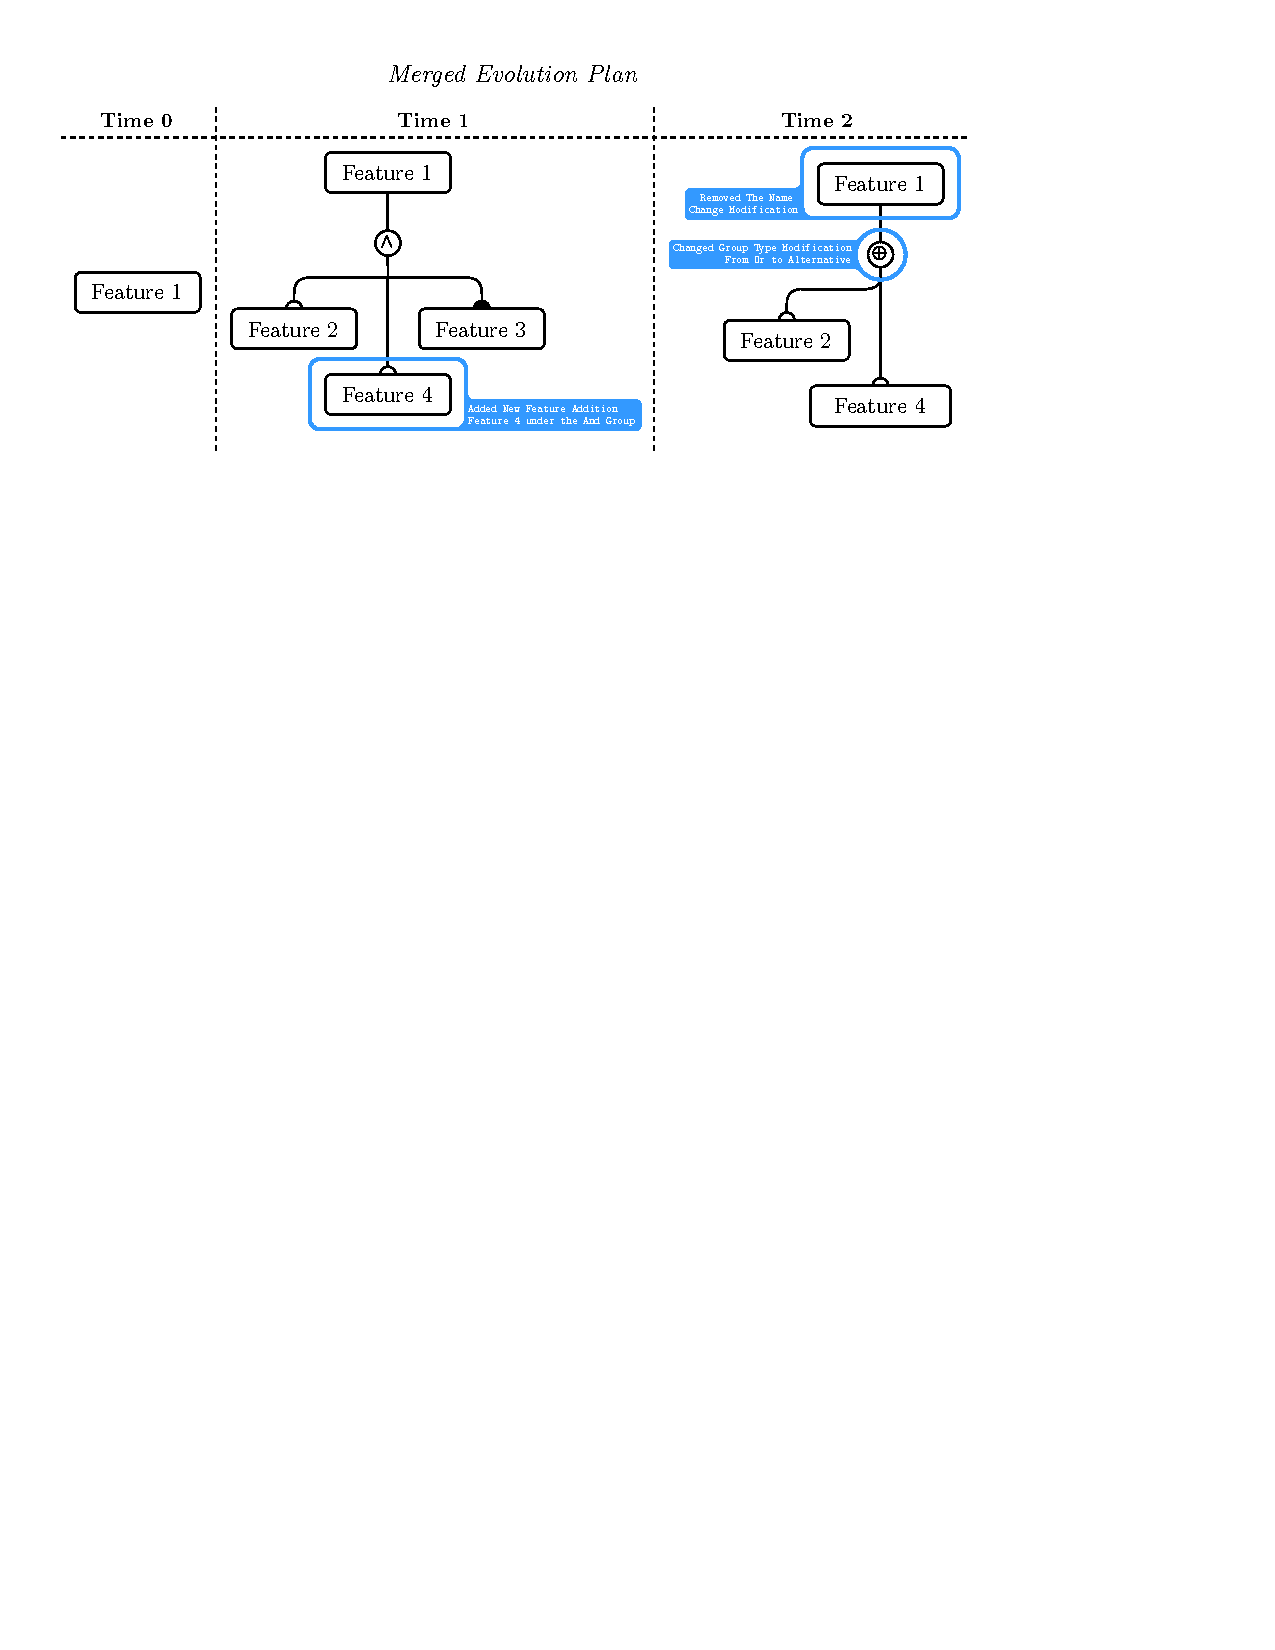
\includegraphics[width=\linewidth]{simple_merged_ep.pdf}
  \caption{A visualization of the merged result of our simple example}%
  \label{fig:simple_three_way_merged_result}
\end{figure}

\chapter{Example Merge – Vending Machine}%
\label{cha:example_merge_vending_machine}

In this chapter, we will apply the three way merge tool on an example inspired from the real world. The example models the evolution of a vending machine software product line. The evolution plan models the planned changes of common vending machine features like beverages such as tea and coffee, different types of currency, different sizes to the cups, etc.

Since we creating a \textit{three} way merge example, we will input three distinct evolution plans to the algorithm. A base evolution plan, and two derived evolution plan, each with their own changes to the base evolution plan. The changes of both versions are then detected and merged into a final, merged version of the evolution plans.

We will showcase two slightly different examples, an example that results in a sound, well-formed evolution plan, and one that results in a conflict. The input to the merge tool is represented in the common serialization format JSON, which is passed as argument to a command line interface wrapping the three-way merge algorithm. The results from the algorithm is then serialized and written to a file. The command line interface will also generate data which is passed to a frontend visualization tool, which visualizes the input and output of the algorithm.

\section{Command Line Interface}%
\label{sec:command_line_interface}

The evolution plan merger defines a command line interface, \texttt{epmerge}, which will do three-way merges on evolution plans. The interface acts as a wrapper around the three-way merge algorithm, handling things like reading and writing to file, logging, converting between representations, etc. 

By designing a command line interface using the common data serialization format json, our application can be easily integrated with other tools. Other tools are often designed and implemented in other technologies and languages, and having a command line interface allows for easier integration of the tools.

We used the Haskell library \textit{optparse-applicative}\footnote{https://github.com/pcapriotti/optparse-applicative} to define the interface, which allowed us to automatically generate a help page. By invoking the command \texttt{epmerge --help}, the following help page will be shown.

\begin{minted}[breaklines]{text}
A three way merge tool for feature model evolution plans

Usage: epmerge ( --generateOne EXAMPLENAME 
               | --generateAll 
               | --fromFile FILENAME
               )
               [-F|--fromType FROMTYPE] [-T|--toType TOTYPE] 
               [-p|--print] [-g|--generateElm] 
               [-o|--toFile FILEPATH]
  Merges evolution plans into a single merged plan, which 
  respects the formal semantics of evolution plans

Available options:
  --generateOne EXAMPLENAME
                        Generates one of the examples
  --generateAll         Generates all examples
  --fromFile FILENAME   Read a three way merge plan from file
  -F,--fromType FROMTYPE   
                        The type to convert from (useful only 
                        when reading from file) (choices: 
                        TreeUser | FlatUser | FlatModification) 
                        (default: TreeUser)
  -T,--toType TOTYPE    The type to convert to (useful when 
                        printing and writing to file) (choices: 
                        TreeUser | FlatUser | FlatModification) 
                        (default: FlatModification)
  -p,--print            Whether to print the merge result
  -g,--generateElm      Whether to pass generated results 
                        to the elm frontend
  -o,--toFile FILEPATH  Outputed file to write the 
                        merge result as JSON
  -h,--help             Show this help text
\end{minted}

\paragraph{Modes}%
\label{par:modes}

The interface has three different \textit{modes}; \texttt{GenerateOne}, \texttt{GenerateAll} and \texttt{FromFile}. The first two will merge either one or all of the predefined test inputs. This includes different variations of the vending machine example we will explore in this chapter. The last, mode \texttt{fromFile}, will read the input from a json encoded file.

The command line interface has three basic `Modes`. `GenerateAll`, `GenerateOne` and `FromFile`.

\begin{itemize}
\item \texttt{GenerateAll} will simply run all the examples in the code. This includes some sound examples and some erroneous examples. The erroneous examples consists of \texttt{Merge} conflicts, \texttt{Local} conflicts and \texttt{Global} conflicts. This mode can be run using \texttt{epmerge --generateAll}.
\item \texttt{GenerateOne} takes one argument, \texttt{Example Name}, which is the string associated with one of the examples in the code. The merger will run the merger on the specified example. This mode can be run using \texttt{epmerge --generateOne EXAMPLENAME}. If you provide an \texttt{EXAMPLENAME} that does not exist, the merger will give you all the available example names.
\item \texttt{FromFile} also takes an argument, \texttt{File Name}, which is the name of json file to read from. The merger will read the file, and run the merger on the input. This mode can be run using \texttt{epmerge --fromFile FILEPATH}.
\end{itemize}

\paragraph{Options}%
\label{par:options}

The interface also defines some optional options that can specify the behaviour of the merge algorithm. The different options will mainly specify the input and output formats, as well as what kind of output will be generated.

When using the \texttt{FromFile} mode, you may specify what evolution plan representation you are using. This can be done with the \texttt{--fromType} option, which takes either \texttt{TreeUser}, \texttt{FlatUser} or \texttt{FlatModification} as a parameter.

In able to view the results of the merge, we could do one or more of the following.

\begin{itemize}
  \item Print the result of the merge using the \texttt{--print} option
  \item Write the result to a json file using the \texttt{--toFile FILEPATH} option.
  \item Write the example(s) to the Elm frontend using the \texttt{--generateElm} option. The next time the frontend is loaded, the user can see an actual visual, tree representation of the \textit{base}, \textit{version 1} and \textit{version 2} evolution plans, as well as the expected and actual merge output. The frontend is discussed in more detail in Section~\vref{sec:a_visualization_tool_for_evolution_plans}.
\end{itemize}

To specify the output format of the print or the file to write the output, you can use the `--toType`, with either `TreeUser`, `FlatUser` or `FlatModification` as an argument.

As an example, running the following will read a sound example from file\footnote{https://github.com/eirikhalvard/master-thesis/blob/master/backend/data/sound\_flatuser.json}, merge the input, and print the result. \texttt{epmerge --fromFile="./data/sound\_flatuser.json" --fromType=FlatUser --print}

\section{A Visualization Tool for Evolution Plans}%
\label{sec:a_visualization_tool_for_evolution_plans}

\todo{elm, files generated from cli. display the eps as a list of trees, with each tree automaticcally drawn using a svg library. designed to help explore the three way merge algorithm, and its inputs and results, svg calculating and drawing each tree to do automatically, showcase a screendump of web page, explaining different elements. used to explore the different examples and edgecases of my tests, note about the visualization tool, how it differs from the paper. mandatory/optional are modeled as colors not dots above the feature. Results are generated and drawn automatically, what we display is simply a screenshot}

\section{A Sound Example}%
\label{sec:a_sound_example}

\todo{sound example. show the base ep. summarize the changes in v1 and v2. changes can be harmonized, show the result}.

\begin{figure}[htpb]
  \centering
  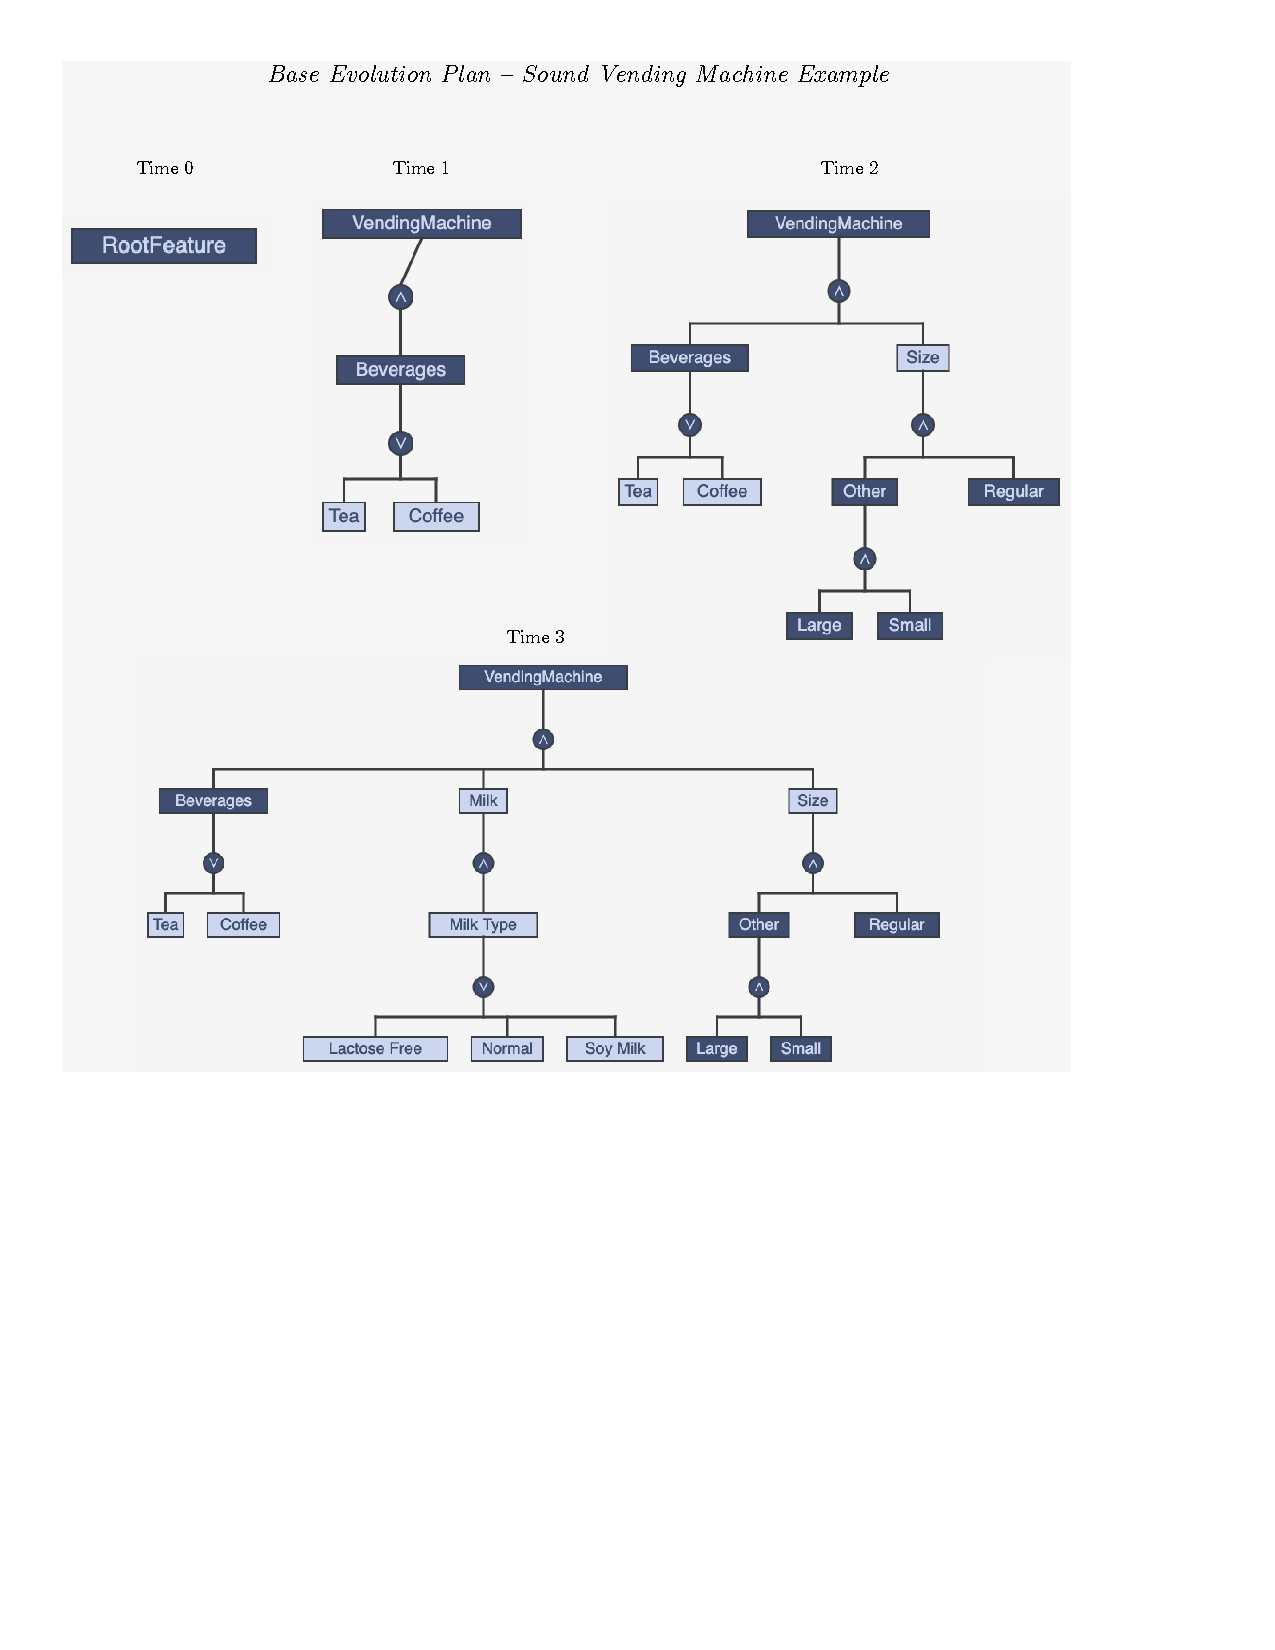
\includegraphics[width=\linewidth]{vending_machine/base_plan.pdf}
  \caption{Sound Vending Machine Example - Base Evolution Plan}%
  \label{fig:vending_machine_sound_base_ep}
\end{figure}

\section{An Unsound Example}%
\label{sec:an_unsound_example}

\todo{unsound example, note that all input eps are sound, this is an assumption. show base ep if not the same as before!. show the base ep. summarize the changes in v1 and v2. maybe say what is different from our sound example. changes cannot be harmonized, show the result}


\todo{OlDTODOwrite about the vending machine example. Write about how the entire example is done. from cli parsing, converting to right representation, merging, checking, converting back, writing to file. Then how the frontend visualization tool parses the result and displays the tree as an interactive thing. sound vs unsound examples}

\chapter{Conclusion and Future Work}%
\label{cha:conclusion_and_future_work}

\todo{konklusjon bør si hvordan det jeg har gjort addresserer forskningsspørsmålene forskningsspørsmålene kan være større en bidraget how to ensure sound plan and merge of sound plans future work kan være flere ting å se på for å belyse forskningsspm}

\backmatter{}

\printbibliography

\end{document}
